\documentclass[10pt]{report}
\usepackage[russian]{babel} 
\usepackage{amsmath}
\usepackage{amssymb}
\usepackage{amsfonts}
\usepackage{amsthm}
\ifx\pdfoutput\undefined
\parindent=1.5cm
\else
\usepackage[pdftex]{graphicx}
\usepackage[unicode, pdftex]{hyperref}
\fi
\hyphenation{words}
\title{Дифференциальные уравнения}
\date{Семинаристы: Степанов Е. О., Матушко М. Г.}
\author {II семестр | Факультет Физики НИУ ВШЭ}
\begin{document}
\maketitle

\tableofcontents
\footnote{Внимание! Конспект написан студентами, и, возможно, содержит смысловые ошибки. При обнаружении ошибок и опечаток пишите на адрес okfazliakhmetova@edu.hse.ru}

\pagestyle {myheadings}
\newpage

\markright{Дифференциальные уравнения. Семинар № 1}
\chapter[{Семинар №1}]{Семинар №1}
\thispagestyle{empty}
\textbf{Задача 1.} Решить дифференциальное уравнение (Задача Коши): 
\newline
\begin{equation}
\hypertarget{1.1}{\dot{U} = \sqrt{U}(U-1)}
\end{equation}
\newline
с начальным условием
\newline
\begin{equation}
\hypertarget{1.2}{U(t_0)=U_0}
\end{equation}\\
\textbf{Решение:} \par
Заметим, что уравнение автономное (правая часть не зависит от времени). \par
Найдем область определения функции:
\[
D: t \in \mathbf{R},   U \in [0; +\infty)  \]
\[ D = \mathbf{R} \times [0; +\infty) \] \par

По теореме Пеано решение существует.

1. $(t_0, U_0) \in \textbf {R} \times (0; +\infty) $\\
 Функция в правой части является непрерывно-дифференцируемой, т. е. решения уравнения не могут пересекаться (по теореме о единственности) -- существует локальная единственность на (0;$+\infty$)  \par
2. Рассмотрим случай, когда U = const. Тогда \[
0 = \sqrt {c}  (c-1)
\] откуда
c = 0  или  c = 1

3. Тогда возможны случаи U $\equiv$ 0 и U $\equiv$ 1 

I) $U_0$  > 1 -- решение  U(.) > 1 [обозначение (.) $\equiv$ для всех t]. Из знака производной следует, что U возрастает.

II) $U_0$ = 1 $\Rightarrow$  U(.) = 1

III) 0 $\leq$ $U_0$ < 1 $\Rightarrow$  0 $\leq$  U(.) < 1. Следует, что U убывает. \par

4. Максимальные интервалы существования решения:

I) 0 < $U_0$ < 1
\[ |f(x, U(x))|  \leq 1 \] $\Rightarrow$ U(.) определено на $\mathbf{R}$ (по теореме о глобальном решении)
\[ U : (-\infty; +\infty) \rightarrow [0;1) \]
По теореме Вейерштрасса:
\[
\lim_{t \to +\infty } U(t) = a
\]
\[
\lim_{t \to -\infty} U(t) = b,
\]
где a и b зависят от начальных условий. Асимптоты a и b у всех траекторий будут одни и те же. Докажем это.
\par
По теореме Лагранжа:
\begin{equation}
\hypertarget{1.3}{ U(k+1)-U(k) = \dot{U}(\xi_k)(k+1-k)}
\end{equation}
Т. к.  $\xi_k \in$ [k, k+1] по теореме о зажатой последовательности $\xi_k$ стремится к +$\infty$, а левая часть \hyperlink{1.3}{(1.3)} стремится к 0, т.к оба слагаемых стремятся к a. Тогда в (1) левая часть стремится к 0, правая -- к $\sqrt{a(a-1)}$, откуда 
\newline a = 0 и a = 1.

У всех этих функций асимптота а = 0, т.к. функция убывает при t $\rightarrow$ +$\infty$.
\newline При t $\rightarrow -\infty$    a = 1, причем касания нет.

II) $U_0$ > 1. Функция возрастает. Возьмем интервал:
\newline
I = ( -$\infty$; $t_0$ + h)

Функция определена на этом интервале. U -- ограничена, следовательно, F -- ограничена. Тогда по теореме о глобальном существовании функция определена глобально на этом интервале. Максимальный интервал существования решений имеет вид
\[
( - \infty; \alpha(t_0, U_0))
\]
Рассмотрим поведение функции при t $\rightarrow$ - $\infty$. Функция будет монотонно убывать, при этом U = 1 она не пересечёт. По теореме Вейерштрасса есть предел (зависящий от начальных условий):
\[
\lim_{n \to -\infty } U(t) = b'
\]
\[
U(k-1)-U(k) = -\dot{U}(\xi)
\]

Левая часть стремится к 0, $\xi$ $\rightarrow - \infty$ по теореме о зажатой последовательности. Тогда $\dot{U} \rightarrow 0, U \rightarrow b'$\\
$\sqrt{b'} (b'-1) = 0$\\
b' = 0 или b' = 1\\
0, очевидно, не подходит. Тогда асимптота 

$\lim_{t \to -\infty } U(t) = 1$

Определить поведение функции справа сложнее. Проинтегрируем \hyperlink{1.1}{(1.1)} с учетом \hyperlink{1.2}{((1.2))}:

\[
\int\limits_{U_0}^U \frac 1 {\sqrt{u}(u-1)}\,du = \int\limits_{t_0}^t \,dT
\]

Заменой в левой части U = $V^2$ и методом неопределенных коэффицентов получаем решение
\begin{equation}
t  - t_0 = \ln\left|\frac {\sqrt{U} -1}  {\sqrt{U} +1}\right| - \ln\left|\frac {\sqrt{U_0} -1}  {\sqrt{U_0} +1}\right|
\end{equation}
Пусть $\ln\left|\frac {\sqrt{U_0} +1}  {\sqrt{U_0} -1}\right|=C$. Тогда выражение (4) принимает вид
\begin{equation}
t  - t_0 = \ln\left|C \frac {\sqrt{U} -1}  {\sqrt{U} +1}\right| 
\end{equation}

Найдем решения $G(u) = F(t)$, где G(u) -- правая часть (5), а  F(t) -- левая.

$I) U_0 > 1 \Rightarrow U(.) > 1$
Решение единственно и удовлетворяет уравнению (5). Мы можем явно выразить U(t):
\[
U = G^{-1}(F(t)) 
\] 

Это выражение верно, когда F(t) лежит в области значений G. \par
Т. е. G((1; +$\infty)) = (-\infty; \ln C).$
\par
а)  t - $t_0$ $\geq$ ln C -- решений нет, т. к. U(t) не определено. \par
b)  t - $t_0$ < ln C $\Rightarrow$
\[
U = \left( \frac {c-exp(t-t_0)} {c+exp(t-t_0)} \right)^2
\]

Отсюда следует, что каждая траектория имеет свой интервал существования, она определена от - $\infty$ до какого-то значения ln(C). Близко к точке  ln(C) решение уходит асимптотически на +$\infty$. 
\par
II) 0 < $U_0$ < 1; 0 $\leq$ U(.) < 1\\
C < 0\\
a) $t-t_0 < ln (-C)$
$U = G^{-1}(F(t)) $\\
G((0; 1)) = (-$\infty$; ln(-C))\\
\[
t  - t_0 = \ln\left|(-C) \frac {\sqrt{U} -1}  {\sqrt{U} +1}\right| 
\]
\[
U=G^{-1}(F(t)) = \left( \frac {c-exp(t-t_0)} {c+exp(t+t_0)} \right)^2
\]
где С < 0. При t $\in$ (-$\infty$; $t_0$ + ln(-C))
\[
t_0 \rightarrow t_0 +ln(-C) - 0
\]
\[
\lim_{t \to {t_0+ln(-C)-0} } U(t) = 0
\]
Вывод: функция в конечный момент времени впадает в 0.

b) При  t - $t_0$ > ln (-C) F(t) не принадлежит области определений G. 
Здесь мы знаем, что решение, равное 0, существует при всех временах.

\bigskip
\textit{Тогда ответ}: \par
\bigskip

a) При U = const U = $U_0$ = 0\\

b) При 0 < $U_0$ < 1:\\
U = 0 для t - $t_0$ $\leq$ ln (-C)\\
U=$\left( \frac {c-exp(t-t_0)} {c+exp(t+t_0)} \right)^2$ для  t - $t_0$ < ln (-C)
\\

c) При U = const U = $U_0$ = 1
\\

d) При $U_0$ > 1:\\
U решений нет для t - $t_0$ $\leq$ ln C\\
U=$\left( \frac {c-exp(t-t_0)} {c+exp(t+t_0)} \right)^2$ для  t - $t_0$ < ln C \par
\bigskip

Графическое решение дифференциального уравнения:

\begin{center}
{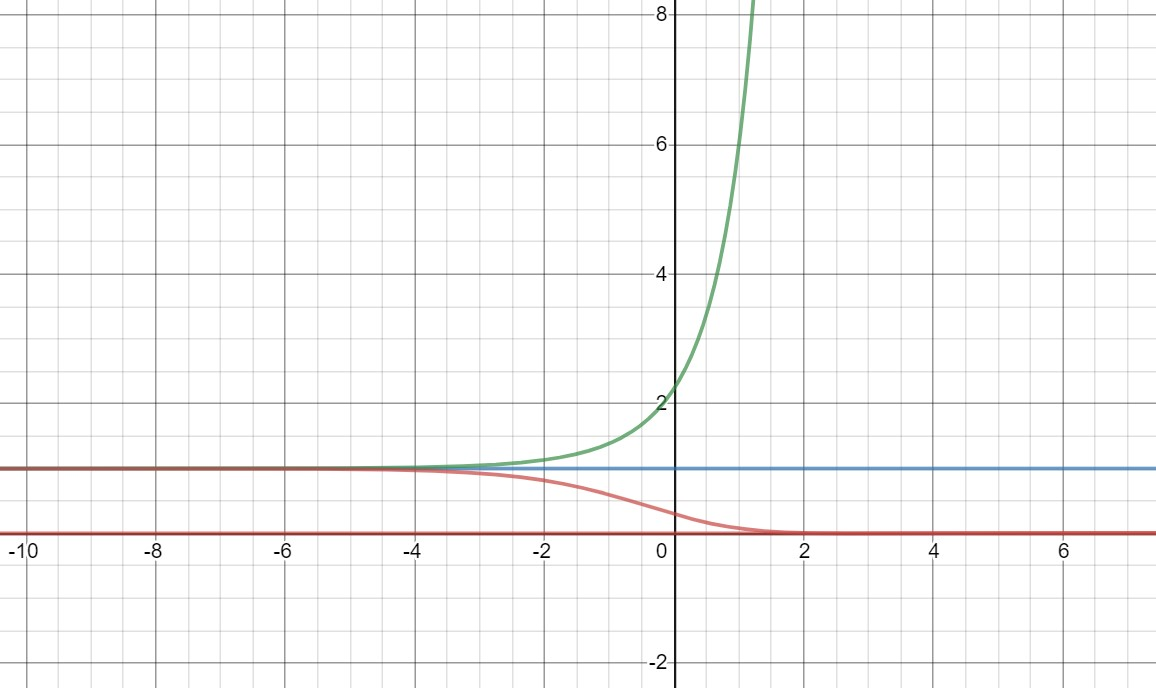
\includegraphics[scale=0.4]{graph1.1.jpg}}
\end{center}

\chapter[{Семинар №2}]{Семинар №2}
\markright{Дифференциальные уравнения. Семинар № 2}
\thispagestyle{empty}
\textbf{Задача 1.} Решить дифференциальное уравнение (Задача Коши): 
\newline
\begin{equation}
\hypertarget{2.1}{\dot{x} = t\left(1+ \frac {1} {x}\right)}
\end{equation}
\newline
с начальным условием
\newline
\begin{equation}
\hypertarget{2.2}{x(t_0)=x_0}
\end{equation}\\
\textbf{Решение:} 

1. Область определения D = $\{ \textbf {R}^2 \backslash x=0\}$

2. Решение локально существует (по теореме Пеано)

3. Из x = const: 
\[
x = -1
\]

4.  В  окрестности любой точки правая часть липщицева -- существует локальная единственность, следовательно, траектории не пересекаются. В частности, никакие траектории не могут пересечь или коснуться $x=-1$. Следовательно, необходимо рассмотреть 3 случая (при этом $t_0$ любое): \[ x_0 < -1, 0> x_0 > -1, x_0 > 0.\]

5. Заметим, что

$y(t) := x(-t)$\\
$\dot{y}(t)=-\dot{x}(-t)=-\left(-t(1+\frac 1 {x(-t)} \right) = t\left(1+ \frac {1} {x}\right)$ -- есть симметрия. Тогда если f(x) является решением, то f(-x) -- тоже решение. Тогда рассматриваем только случай t>0. 

6. Монотонность\\
\[
\ddot{y} = 1+1/x + t*\left(- \frac {\dot{x}} {x^2}\right)=(1+1/x)- \frac {t^2} {x^2} (1+1/x)= \frac {(x+1)(x-t)(x+t)} {x^3}
\]
Вторая поизводная поможет определить промежутки вогнутости функции. 
На рисунке изображены знаки производной и промежутки вогнутости.
\begin{center}
{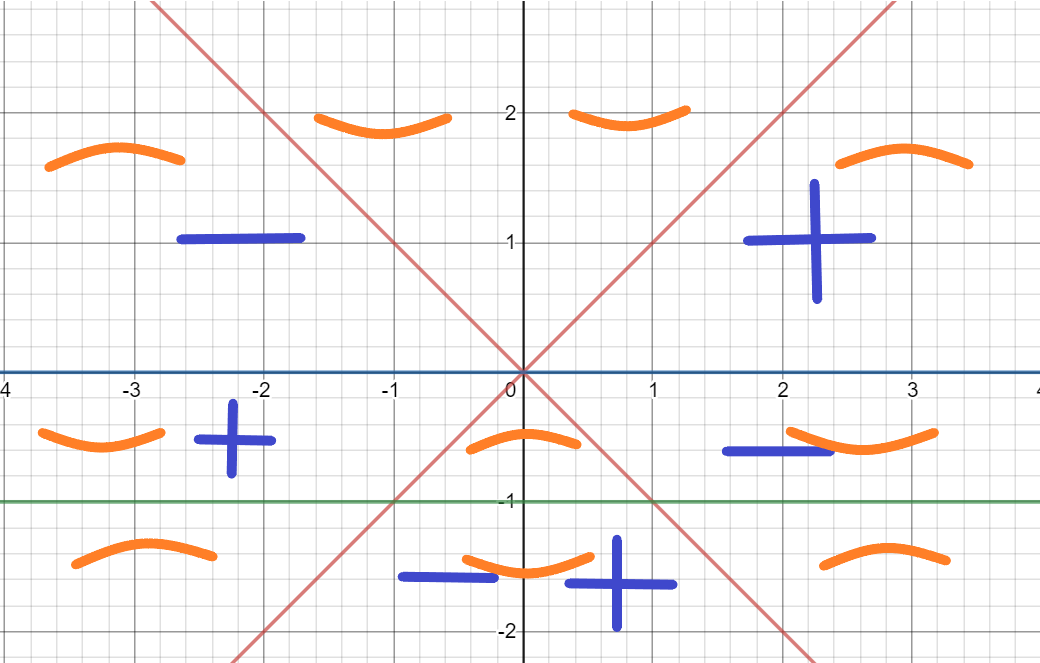
\includegraphics[scale=0.45]{graph2.2.png}} 
\end{center}

Проинтегрируем выражение (Можем сделать это, в отличие от задачи №1 первого семинара, не потеряв никаких решений. Решение могло бы входить в -1, но мы знаем из теоремы о единственности, что такого не будет):
\[
\frac {dx} {1+x} x = tdt 
\]
Получаем выражение
\[
x-ln|x+1| = \frac {t^2} 2 - \frac {t_0^2} 2 +G(x_0)
\]
Обозначим  $\frac {t^2} 2- \frac {t_0^2} 2 +G(x_0) = F(t)$, $G(x)=x-ln|x+1|$ \\
Функция G(x) меняет знак, не монотонна, и потому не допускает обратной функции. Поэтому необходимо рассматривать разные интервалы.\\

Случай 1.\\
$x_0>0 \Rightarrow x(t)>0$\\
Функция возрастает на этом интервале. Минимум -- в 0, G(0) = 0,\\
G($\infty$) $\rightarrow$ +$\infty$ \\
G((0; +$\infty$))=(0; +$\infty$)\\
G(x) =  F(t). Уравнение обратимо, когда F(t) принадлежит образу G(x).  Смотрим положительные t (в отрицательных -- симметрично):

F((0; +$\infty))=(-\frac {t_0^2} 2 +G(x_0); +\infty$)

1. 1) \[-\frac {t_0^2} 2 +G(x_0) \ge 0 \Rightarrow\] решение существует для всех t.

1. 2) \[-\frac {t_0^2} 2 +G(x_0) < 0
\]\[
F((0; +\infty))=G(0; +\infty)\]
Тогда существует решение на интервале  ($-\infty; -\overline{t})$  в объединении с  ($\overline{t}; +\infty)$, где\\
$\overline{t} = \sqrt{t_0^2-2G(x_0)}, \overline{t} = \overline{t}(t_0, x_0)$\\

Нарисуем кривую, разделяющую эти решения: $\frac {t_0^2} 2 = x_0 - ln(x_0+1)$
\begin{center}
{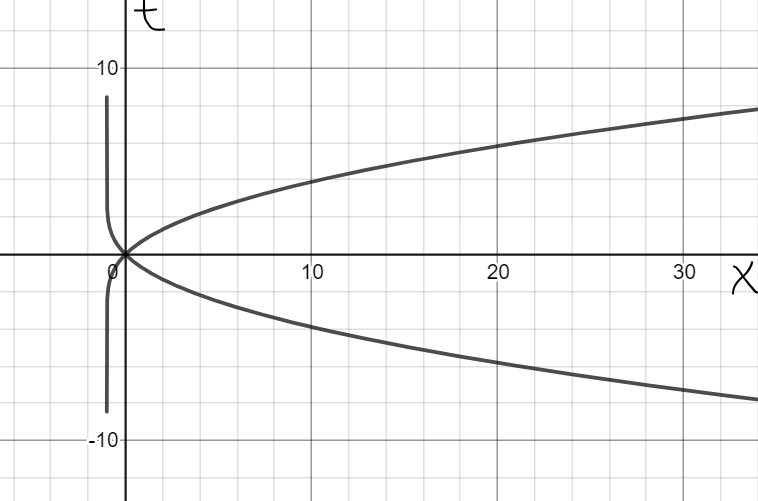
\includegraphics[scale=0.5]{graph2.3.png}} 
\end{center}
Она является сепаратрисой двух случаев. Точки выше кривой соответствуют 1.2), точки на кривой и выше 0 -- случай 1.1). \\
При x $\Rightarrow +\infty$  $G(x) \approx x.\\
 x = t^2/2 + C $ (при больших x решение -- примерно парабола) \\

Случай 2.\\
$x_0 \in (-1; 0) \rightarrow x(t) \in (-1; 0)$\\ 
 Производная G отрицательна, функция убывает монотонно, минимум в 0 равен 0. При x $\rightarrow -1$ функция стремится к  $+\infty$:\\
$G((-1; 0))  = (0; +\infty)$ \\

График G(x) на (-1;0):
\begin{center}
{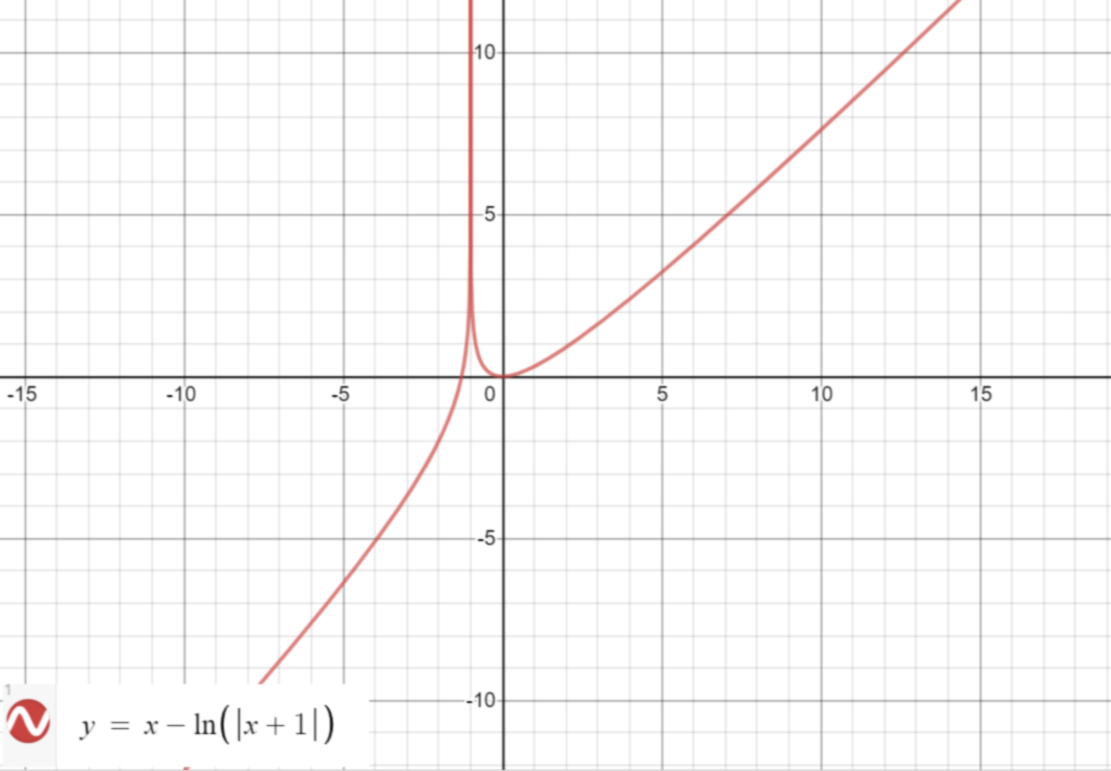
\includegraphics[scale=0.5]{graph2.4.png}} 
\end{center}

2.1) \[-\frac {t_0^2} 2 +G(x_0) \ge 0\] решения существуют для всех t.

2.2) \[-\frac {t_0^2} 2 +G(x_0) < 0\]  
Далее -- аналогично случаю 1.\\

Случай 3.
\[ 
x_0 \in (-\infty; -1) \]
\[
G((-\infty; +\infty))=(-\infty; +\infty)
\]
Решение существует для любых t.

Рассмотрим поведение графика для случая 1) на бесконечности:\\
$\dot{x}=t(1+1/x)>t$\\
 $\dot{x}>t$\\
\[x(t) > x_0 + \frac {t^2-t_0^2} 2 \] 
это неравенство Чаплыгина. Получается, что траектория выше, чем парабола $x_0 + \frac {t^2-t_0^2} 2$. Асимптоты нет, и функция растет быстрее чем квадрат. 

Графическое решение дифференциального уравнения x(t):
\begin{center}
{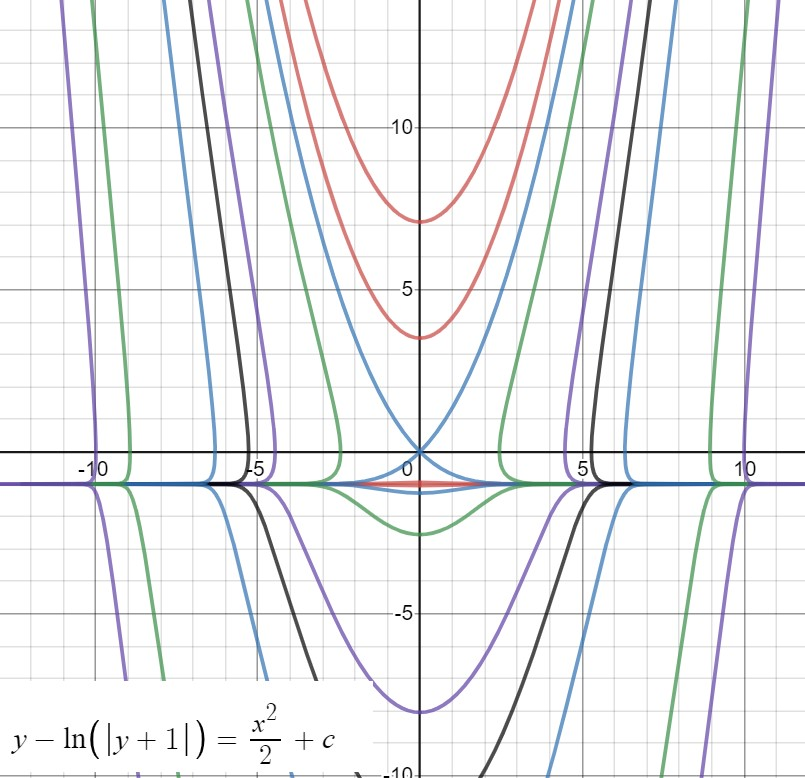
\includegraphics[scale=0.45]{graph2.4.jpg}} 
\end{center}
\textbf{Задача 2.} Решить дифференциальное уравнение (Задача Коши): 
\newline
\begin{equation}
\hypertarget{2.3}{\dot{x} =  \frac {2t+x} {t-2x}}
\end{equation}
\newline
с начальным условием
\newline
\begin{equation}
\hypertarget{2.4}{x(t_0)=x_0}
\end{equation}\\
\textbf{Решение:} \par
1) Область определения D = $\{ \textbf {R}^2 \backslash x=t/2\}$

2) Локальная единственность есть, локальное существование есть, траектории не пересекаются.

3) Интервалы монотонности и выпуклости

4)Попробуем явно решить (2.3). Заметим, что уравнение однородно\\
$\dot{x} =  \frac {2+x/t} {1-2x/t}$. Случай t = 0 необходимо рассмотреть позже.

5)Сделаем замену U =x/t, x=tU\\
\[
\dot{x} = U+ t\dot{U}
\]
\[
 U+ t\dot{U} = \frac {2+U} {1-2U}
\]
\[
\dot{U} = \frac {2(1+U^2)} {t(1-2U)}
\]
\[
\frac {dU(1-2U)} {1+U^2} = \frac {2dt} t
\]
После интегрирования получаем
\[
arctg(U)-ln(1+U^2)=ln(ct^2)
\]
\[
ct^2=\frac {exp(arctg(U))} {1+U^2}\]
Теперь мы можем решить уравнение относительно U(t), а потом перейти к x(t)


\chapter[{Семинар №3}]{Семинар №3}
\markright{Дифференциальные уравнения. Семинар № 3}
\thispagestyle{empty}
\textbf{Задача 1.} Решить дифференциальное уравнение (Задача Коши): 
\newline
\begin{equation}
\hypertarget{3.1}{\dot{y} =  \frac {x+y} {x-y}}
\end{equation}
\newline
с начальным условием
\newline
\begin{equation}
\hypertarget{3.2}{y(x_0) = y_0}
\end{equation}\\
\textbf {Решение}

1) D = \textbf{R} $\{\backslash$ x = y\}. Локальное существование есть

2) Производная непрерывна в области определения, в окрестности любой точки $x_0, y_0$ производная ограничена, значит, функция локально липщицева, локальная единственность есть, траектории не пересекаются. (по теореме о единственности)

3) Знаки производной:
\begin{center}
{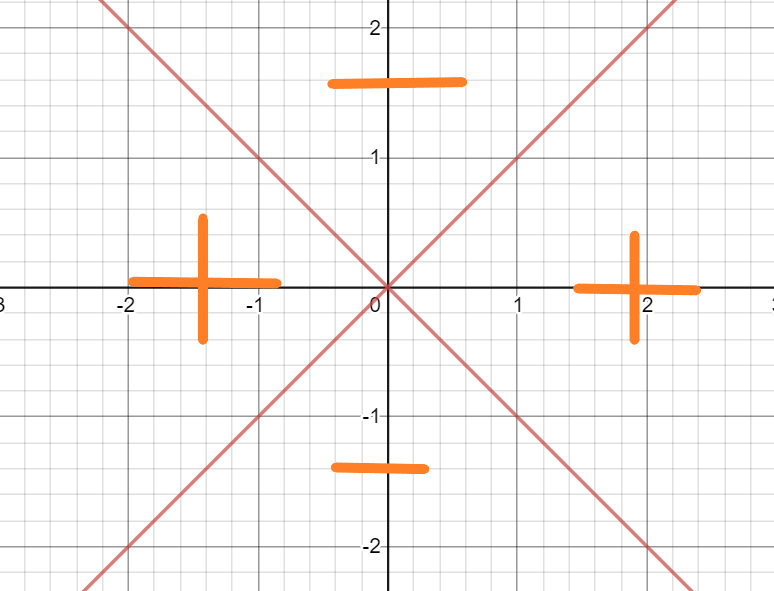
\includegraphics[scale=0.4]{graph3.1.png}} 
\end{center}

Обратим внимание, что на прямой $x = - y$ производная равна нулю. На ней находятся максимумы (выше (0,0)) и минимумы (ниже (0,0)) траекторий.  В точках пересечения с этой прямой график будет иметь горизонтальную касательную. 

Присутствует симметрия относительно начала координат \[
z(x)  =-y(-x)\]
\[
z'= y'(-x) = \frac {-x+y(-x)} { -x - y(-x)} = \frac {-x-x(x)} {x+z} {x-z}\]\\


Заметим, что уравнение однородно. Тогда  
\[ y' = \frac {1+y/x} {1 - y/ x}\]
\[
U := y/x\]
\[
y(x) = xU(x)\]
\[y' = U(x) + xU'(x)= \frac {1+U} {1-U}\]\[
xU'(x) = \frac {1+U} {1-U} - U = \frac {1+U^2} {1 - U}\]
Получили уравнение с разделяющимися переменными (Можем поделить на x, ведь в уравнении выше при x = 0 левая часть 0, а правая в 0 никогда не обращается. В исходном же уравнении необходимо рассмотреть случай x =0):
\[
\frac {dU(1-U)} {1+U^2} = \frac {dx} {x}\]
Проинтегрируем и введем обозначения:
\[
F(U) = arctg (U) - \frac 1 2 ln(U^2 +1)\]
Построим график F(U). Знаки производной мы уже знаем. Производная меняет знак в U = 1. Подстановкой в F(U) найдем максимум функции. Рассмотрим поведение функции на бесконечности. При U $\rightarrow +\infty$ функция ведет себя как $-ln|U|+\pi/2$, при U $\rightarrow -\infty$ как $  -ln|U|- \pi/2$
\begin{center}
{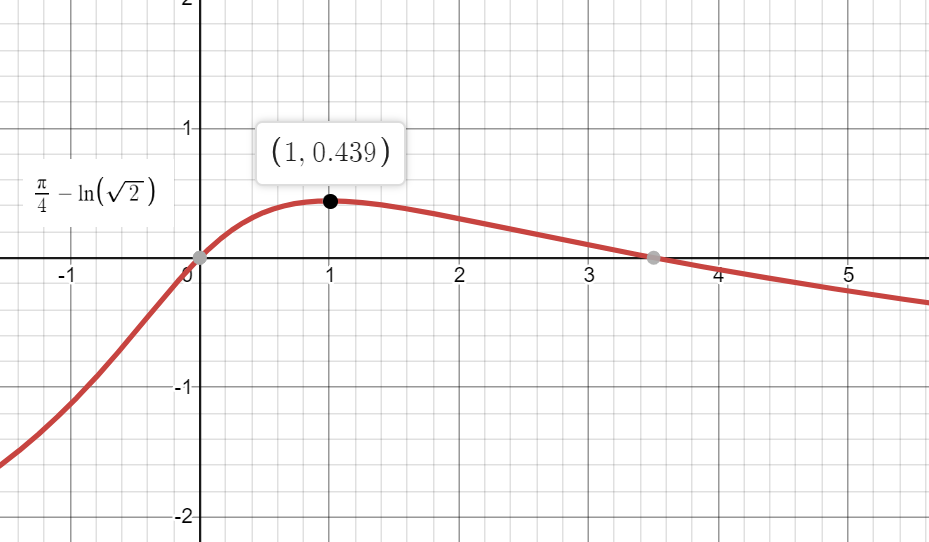
\includegraphics[scale=0.48]{graph3.2.png}} 
\end{center}
С учетом наших обозначений
\[
F(U)-F(U_0) = ln|x|-ln|x_0|\]
\[
F(U) = ln|x| + F(U_0) - ln|x_0|\]
Обозначим $ F(U_0) - ln|x_0| =: ln(C)$ и $C  = C (x_0, y_0)>0$
\\
Тогда необходимо решить следующее уравнение для всех начальных данных:
\begin{equation}
\hypertarget{3.3}{F(U) = lnC|x|}
\end{equation}

Найдя корни этого уравнения, мы найдем два возможных решения: одно соответствует U < 1, другое для U > 1. Эти решения соответствуют разным траекториям, по разные стороны от прямой y = x. Из теоремы о единственности (см. пункт 2) других решений нет. Таким образом, мы найдем абсолютно все решения. \hyperlink{3.3}{(3.3)} разрешимо, когда область определения 
\[
lnC|x| \leq \pi/4 - ln \sqrt{2}\]\[
C|x| \leq e^{\pi/4 - ln \sqrt{2}}\]
\[
- \frac 1 {c\sqrt{2}} e^{\pi/4} \leq x \leq \frac 1 {c\sqrt{2}} e^{\pi/4} \] -- нашли интервал существования, и он ограничен. Все решения существуют только на нем.
Рассмотрим случай, когда $x \rightarrow \pm \frac 1 {c\sqrt{2}} e^{\pi/4} $. Подставив в \hyperlink{3.3}{(3.3)}, увидим, что U = 1. Однако этот случай не удовлетворяет области определения \hyperlink{3.1}{(3.1)}. Значит, при $x \rightarrow \pm \frac 1 {c\sqrt{2}} e^{\pi/4}$ $ y \rightarrow x $. Подставив это значение в производную \hyperlink{3.1}{(3.1)}, увидим, что она стремится к бесконечности, из чего следует, что траектория попадает туда вертикально. Кроме того, интервал существования начального уравнения открытый, неравенства на x строгие. Таким образом, можем построить график решений:
\begin{center}
{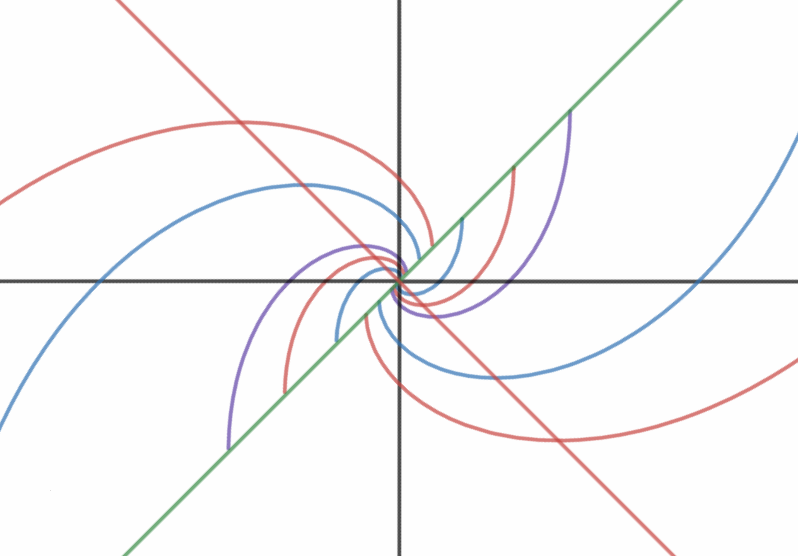
\includegraphics[scale=0.5]{graph3.3.png}} 
\end{center}
\newpage
\section {Линейные уравнения}
 \textbf{Задача 2.} Решить дифференциальное уравнение (Задача Коши): 

\begin{equation}
\hypertarget{3.4}{\dot{y} = 2xy -1 }
\end{equation}
\newline
с начальным условием
\newline
\begin{equation}
\hypertarget{3.5}{y(x_0) = y_0}
\end{equation}\\
\textbf {Решение:}

Уравнение линейно по y\[
y(x) = U(x)V(x)\] -- стандартный способ найти решение уравнения
\[
y' = U'V+UV' = 2xUV -1 \]
\[
V(U'-2xU)+V'U = -1\]
Мы можем выбрать функцию U любой. Выберем ее такой, чтобы выполнялось следующее равенство. Важно, что нам нужно найти любое решение (не все):
\[ U'-2xU = 0\]
Уравнение с разделяющимися переменными. Его решение:
\[U = exp(x^2)\]
Вернемся к нашему уравнению:
\[
V'exp(x^2) = -1\]
\[ V' = -exp(-x^2)\]
Получили уравнение, которое не решается при помощи сведения к элементарным функциям. Тогда
\[
V (x) = \int\limits_{x_0}^x e^{-s^2} ds + C
\]\[
y = UV = e^{x^2}\left(- \int\limits_{x_0}^x  e^{-s^2} ds + C \right) \]
\textit{Домашнее задание: дорешать, нарисовать траектории и исследовать}

\vspace{15mm}
 \textbf{Задача 3.} Решить дифференциальное уравнение (Задача Коши): 
\newline
\begin{equation}
\hypertarget{3.5}{\dot{x} =x^2 - t^2-1}
\end{equation}
\newline
с начальным условием
\newline
\begin{equation}
\hypertarget{3.6}{x(t_0) = x_0}
\end{equation}\\
\textbf {Решение:}

$1) D= \textbf{R}^2 $

2) Непрерывна, локально существует везде (в силу теоремы Пеано)

3) Траектории не пересекаются.

4) Монотонность.\\
Посмотрим на знак производной;
$\dot{x} > 0$, когда $x > \sqrt{t^2+1}$ и $x <- \sqrt{t^2+1} $\\ -- график является гиперболой. 
\begin{center}
{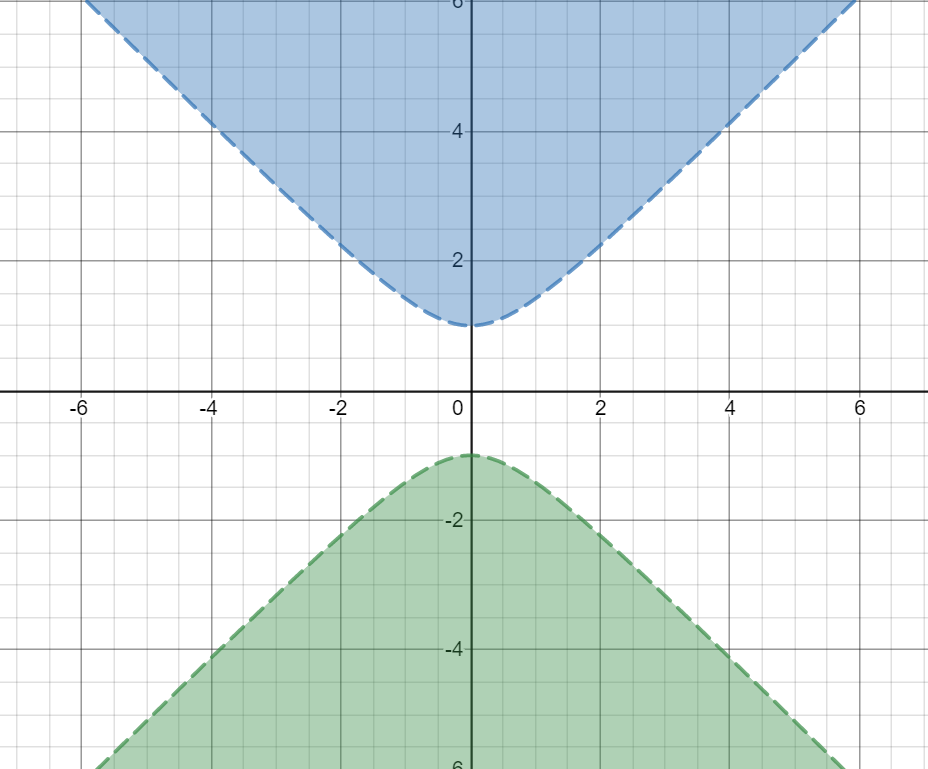
\includegraphics[scale=0.45]{graph3.4.png}} 
\end{center}
Закрашенные промежутки -- производная > 0, функция возрастает, незакрашенные -- убывает. Пересечение ветвей гиперболы возможно только горизонтально (производная на ветвях = 0)

Одно решение угадывается сразу: $x = -t$. Заметим, что никакая другая траектория ее пересечь не может.\\
$x(t) = V(t) - t$ -- отнимаем решение. Тогда это решение в терминах полученного уравнения будет стационарным.\\
\[
\dot{x} = \dot{V} - 1
\]
\[ \dot{V} - 1= (V-1)^2 - t^2-1 = V^2 - 2Vt -1 
\]
\[
\dot{V} = V^2 -2Vt\]
Обратим внимание, что здесь есть решение V=0, что соответствует в начальном уравнении $x = -t$. Сделаем замену:
\[
V = \frac 1 U\]
\[
\dot{V} = - \frac {\dot{U}} {U^2} = \left(\frac 1 U\right)^2 - \frac {2t} U\]
\[
\frac {\dot{U}} {U^2} =  \left(\frac 1 U\right)^2 - \frac {2t} U\]
\[
\dot{U}= 2Ut - 1\]  получили линейное уравнение (см. задачу 2)

Из 2-й задачи:\[
U =  e^{t^2}\left(- \int\limits_{t_0}^t  e^{-s^2} ds + C \right) \]
Необходимо перейти обратно к x:
\[
x(t) = \frac {e^{t^2}} {- \int\limits_{t_0}^t e^{-s^2} ds + C} - t\]
Найдем С:
\[
x_0 = x(t_0) = \frac {e^{t_0^2}} {C} - t_0\]
Откуда $ C =  \frac {e^{-t_0^2}} {x_0+t_0} $

Определим максимальный интервал существования решения. Область определения не содержит все \textbf{R}, когда зануляется знаменатель. Рассмотрим возможные случаи:

(i). Известно, что  $\int\limits_{t_0}^t e^{-s^2} ds$ не превосходит $\sqrt{\pi}$. Тогда если  $ C =  \frac {e^{-t_0^2}} {x_0+t_0}  > \sqrt{\pi}$ -- знаменатель не зануляется

(ii). $t< t_0 $ -- знаменатель всегда > 0 (из свойства граничных условий интеграла).
$ (-\infty; t_0] $ содержится в любом максимальном интервале существования

(iii). Тогда возможны 2 случая:

(*) Существует $\overline t>t_0$:
\[
\frac {e^{-t_0^2}}{x_0+t_0}=  \int\limits_{t_0}^{\overline{t}}  e^{-s^2} ds\]
Решение определено на $(-\infty; \overline t)$

(**) Такого $\overline t $ нет\\
Знаменатель не зануляется. Решение определено на \textbf{R}

(iiii) Рассмотрим оба решения при t на бесконечности:

а) При $t \rightarrow -\infty$:\\
Знаменатель не зануляется, стремится к положительному числу. Числитель стремится к 0.
x(t)+t $\rightarrow$ 0 -- в обоих случаях. Тогда $x = -t$ -- асимптота. Тогда есть одно пересечение с гиперболой, иначе функция в верхней части гиперболы неограниченно возрастает и не может иметь асимптоту $x = -t$.

б) $ t \rightarrow \overline t-0$\\
$x(t) \rightarrow +\infty)$ -- у каждой траектории своя асимптота. Лишь одно пересечение с гиперболой

в) (iii.(**)) $t \rightarrow +\infty$\\
x(t)+t $ \rightarrow 0$

Рассмотрим отдельно случай (i) $\frac {e^{-t_0^2}}{x_0+t_0}> \sqrt{\pi}$\\
$ x_0+t_0 < \frac {e^{-t_0^2}}{\sqrt{\pi}}$. Тогда решения:
\begin{center}
{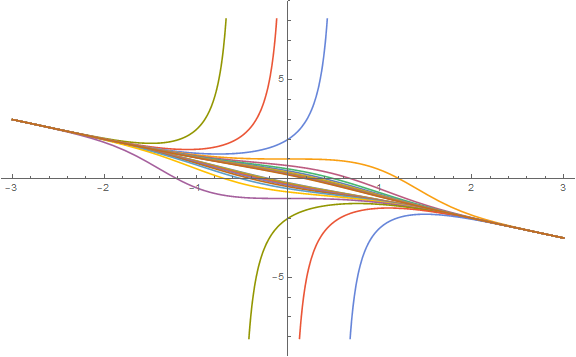
\includegraphics[scale=0.7]{graph3.5.png}} 
\end{center}

\chapter[{Семинар №4}]{Семинар №4}
\markright{Дифференциальные уравнения. Семинар № 4}
\thispagestyle{empty}
\textbf{Задача 1.} Решить дифференциальное уравнение (Задача Коши): 
\newline
\begin{equation}
\hypertarget{4.1} {y' -  \frac {2y} {x+1} = (x+1)^2}
\end{equation}
\newline
с начальным условием
\newline
\begin{equation}
y(x_0) = y_0
\end{equation}\\

\textbf {Решение:}\\
Перепишем (4.1) как
 \[y' = - \frac {2y} {x+1} + (x+1)^2\]
1) Область определения правой части:
\[ D = \{(x,y) \in \textbf{R} \backslash x = 1\}\]

2) Правая часть непрерывна, локальное существование есть. Уравнение -- линейное по y. Интервал существования решения для линейных уравнений максимально возможный.

3)  Интегрвалы существования решения:\\
$x_0 > -1, x(.) $ определен на $(-1; +\infty)$;  $ x_0 < -1, x(.) $ определен на $(-\infty; -1)$

4) Интервалы монотонности. Найдем $y'>0$\\
\[ \frac {2y} {x+1} +(x+1)^2>0\]

4.1) Случай $x > -1$\\
\begin{equation}
y > - \frac {(x+1)^3} {2} 
\end{equation}

4.2) Случай $ x<-1$
\begin{equation}
y < - \frac {(x+1)^3} {2} 
\end{equation}
Знаки производной изображены на графике.
\begin{center}
{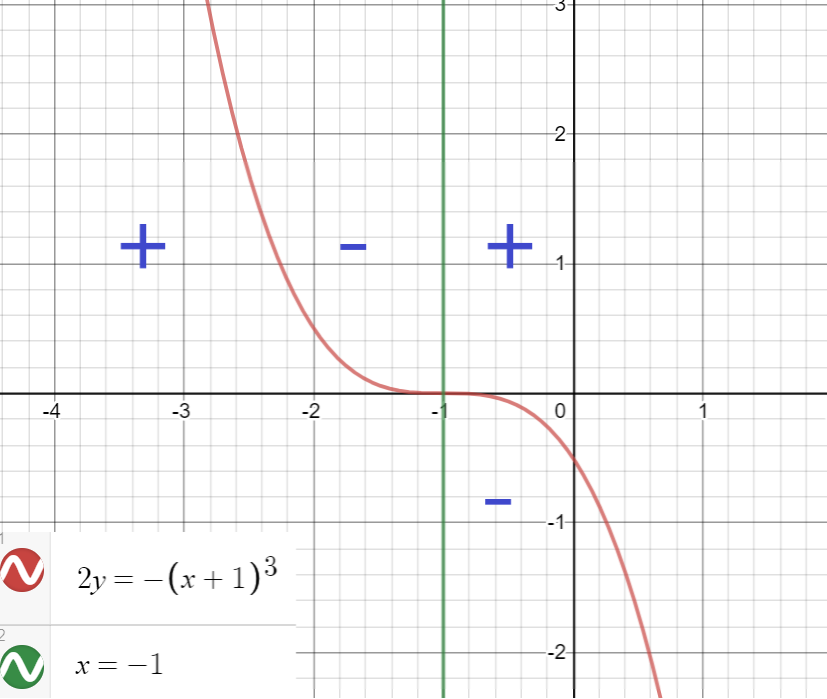
\includegraphics[scale=0.45]{graph4.3.png}} 
\end{center}

5. Выпуклость:\\
\[ y'' - \frac {2y'} {x+1} + \frac {2y} {(x+1)^2} = 2(x+1)\]
\[ y'' - \frac {2} {x+1}\left((x+1)^2+\frac {2y} {x+1}\right) + \frac {2y} {(x+1)^2} = 2(x+1)\]
\textit{Упражнение}. Найти промежутки выпуклости функции.

6. Сделаем замену $y = UV$. \\
\[ y' = U'V+V'U\]
\[  U'V+V'U - \frac {2UV} {x+1} = (x+1)^2\]
\begin{equation}
\hypertarget{4.5} {V\left(U'-\frac {2U}{x+1}\right)+V'U = (x+1)^2}
\end{equation}
Выберем функцию U такую, что $ U'-\frac {2U} {x+1} = 0$
\[ U'=\frac {2U} {x+1}\]
\[ \frac {dU} {U} = \frac {2dx} {x+1}\]
\[ ln(U) = ln(x+1)^2\]
\[U=(x+1)^2\]
Подставим U в  \hyperlink{4.5}{(4.5)} и найдем V:
\[V'(x+1)^2=(x+1)^2\]
\[ V' = 1\] 
\[ V = x+C\]
\[y = VU = (x+1)^2(x+C)= (x+1)^2(x+1+C) = (x+1)^3+C(x+1)^2\]
(Обратите внимание на то, что C в первом и втором переходе -- разные константы). Определим С из начальных условий:
\[(x_0+1)^3+C(x_0+1)^2=y_0\]
\[C = \frac {y_0} {(x_0+1)^2} - (x_0+1)\]

7) Построим график решений. В зависимости от начальных данных, выделим 2 случая: $x_0 > -1$ и $x_0 < -1$.

$7.1) x_0 > -1$\\
Пусть x$\rightarrow +\infty$. Т.к третья степень растет быстрее квадрата:
\[ y \approx (x+1)^3\]
Рассмотрим x$\rightarrow -1$: y$\rightarrow 0$. При этом $(-1;0)$ исключена.\\
$y' = 3(x+1)^2+2C(x+1)- $ касательная горизонтальна в 0.

$7.2) x_0 < -1$\\
Аналогично, пусть x$\rightarrow -\infty$:
\[ y \approx (x+1)^3\]
При x$\rightarrow -1$: y$\rightarrow 0$\\
$y' = 3(x+1)^2+2C(x+1)- $ касательная горизонтальна в 0.

Тогда график решений уравнения \hyperlink{4.1}{(4.1)} выглядит так:
\begin{center}
{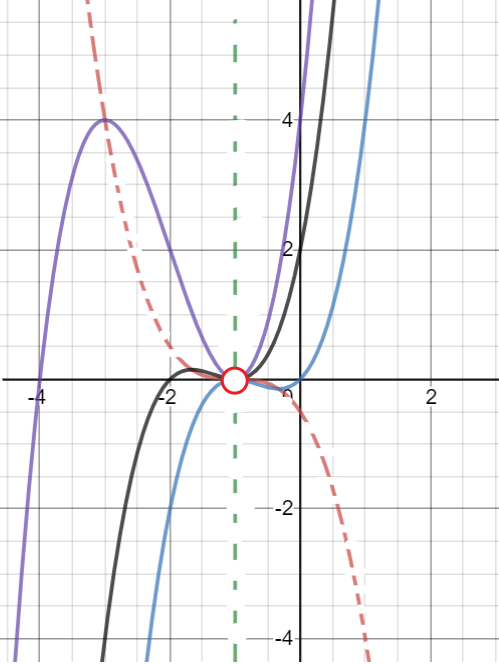
\includegraphics[scale=0.45]{graph4.4.png}} 
\end{center}

\vspace{15mm}
\textbf{Задача 2.} Решить дифференциальное уравнение (Задача Коши): 
\newline
\begin{equation}
\hypertarget{4.6}{y'\left(\frac {y^2-3x^2}{y^4} \right) +\frac {2x} {y^3} = 0}
\end{equation}
\newline
с начальным условием
\newline
\begin{equation}
y(0) = 1
\end{equation}

\textbf {Решение:}
\begin{equation}
\hypertarget{4.8}{ y' = -\frac {2xy}{y^2-3x^2}}
\end{equation}

1) Обратим внимание, что \hyperlink{4.6}{(4.6)} и \hyperlink{4.8}{(4.8)} имеют разные области определения. Правая часть \hyperlink{4.8}{(4.8)} не определена на $y^2=3x^2$, а \hyperlink{4.6}{(4.6)} -- на $y=0$.

2) Определим знаки производной:
\begin{center}
{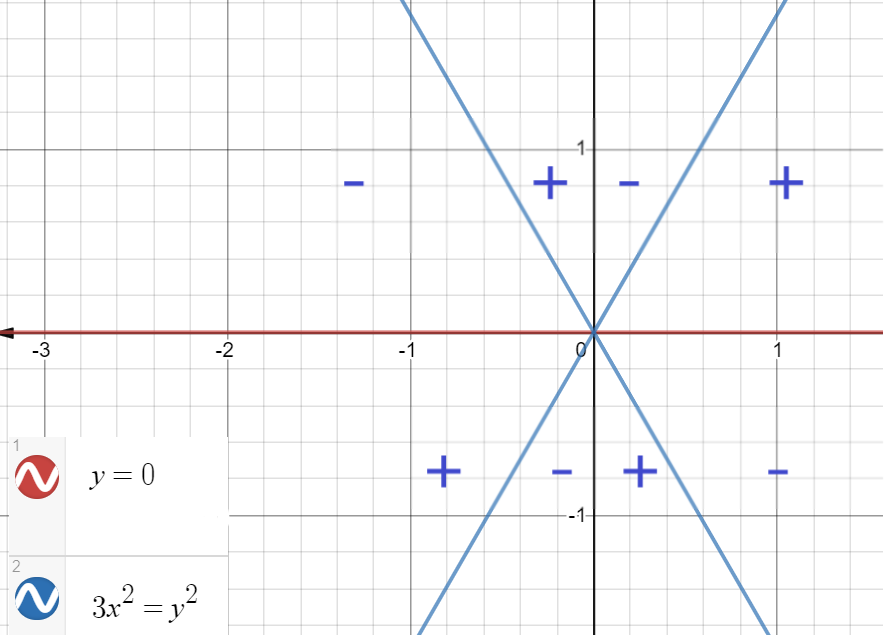
\includegraphics[scale=0.4]{graph4.2.png}} 
\end{center}

3) Перепишем \hyperlink{4.6}{(4.6)} в следующем виде:
\begin{equation}
\hypertarget{4.9}{\frac {2x} {y^3}dx + \frac {y^2-3x^2} {y^4} dy = 0}
\end{equation}\\
В таком виде равенство напоминает полный дифференциал:
\[ df = f_x dx +f_y dy\]
Предположим, что \hyperlink{4.9}{(4.9)} является полным дифференциалом какой-то функции.
Тогда для этой функции должно выполняться
\[ \frac{\partial f}{\partial x}=f_x = \frac {2x} {y^3}\]
\[\frac{\partial f}{\partial y} = f_y = \frac{y^2-3x^2} {y^4}\]
Необходимое условие: если найденная функция гладкая, то $f_{xy}=f_{yx}$. Проверим выполнение для \hyperlink{4.9}{(4.9)}.

\[f_{xy} = \left( \frac {2x} {y^3}\right)'_y = -\frac {6x} {y^4}\]
\[f_{yx} = -\frac {6x} {y^4}\] 
Действительно, $ f_{yx} = f_{xy}$, но из этого не следует, что такая f существует (это лишь необходимое условие, но недостаточное). Несмотря на это из $ f_{yx} = f_{xy}$ следует, что мы можем построить такую функцию в маленькой окрестности каждой точки (по лемме Пуанкаре)
\[ \frac {df} {dx} = \frac{2x}{y^3}\]
Интегрируя, получим
\[ f = \frac {x^2} {y^3} +C(y)\]
Возьмем производную по y:
\[ f_y = -\frac {3x^2} {y^4}+C'(y)\]
Кроме того, $f_y = \frac{y^2-3x^2} {y^4}$. Приравняем:
 \[ \frac {y^2} {y^4}-\frac {3x^2} {y^4} = -\frac {3x^2} {y^4} + C'(y)\]
\[
C'(y) = \frac {1} {y^2}\]
Отсюда следует, что (D = const):
\[ C(y) = -\frac {1} {y}+D\]
\[ f(x, y) = \frac {x^2} {y^3}-\frac {1} {y}+D\]
Для \hyperlink{4.9}{(4.9)}  f(x, y) = 0. Это значит, что f сохраняется вдоль любой траектории
\[ \frac {x^2} {y^3}-\frac {1} {y} = C\]
Отсюда следует, что всюду (кроме прямых $y^2=3x^2$ и y = 0) существует единственность. 
Найдем константу для наших начальных условий:
\[ y (0) = 1\]
\[ C=-1\]

4) Вспомним, что $y> 0$
\[ \frac {x^2} {y^3}-\frac {1} {y} = -1\]
\[x^2=y^2-y^3\]
\[F(y):=y^2-y^3\]
Т.к. $ y > 0, y_{max}= 2/3, F_{max}=4/27$
\begin{center}
{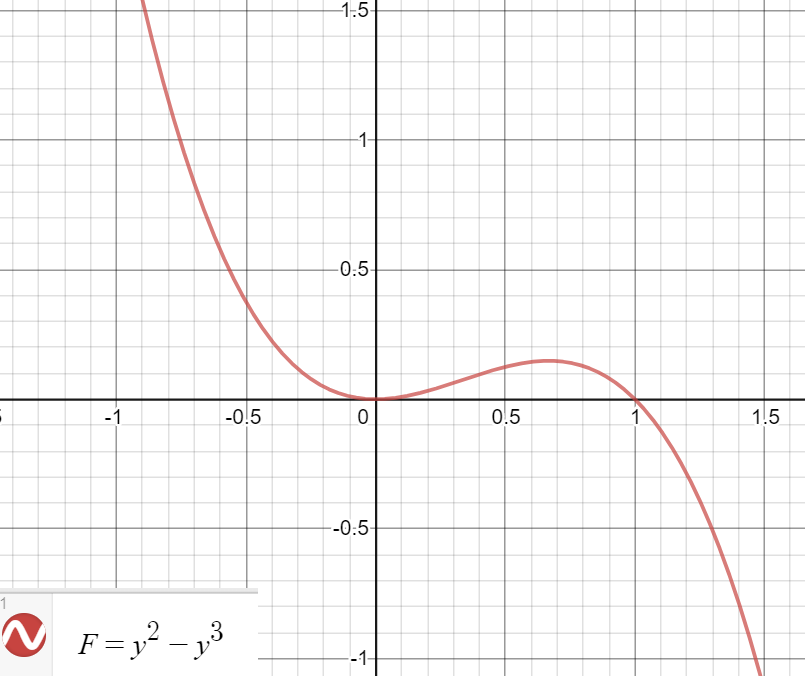
\includegraphics[scale=0.4]{graph4.5.png}} 
\end{center}
$y(0) = 1$. Поэтому мы рассматриваем ветвь графика y > 2/3
\[y = F^{-1} (x^2)\]
$x^2$ должен лежать в области значений F:
\[
x^2 \leq 4/27\]
\[ x \in [-2/3\sqrt{3};2/3\sqrt{3}]\]
Рассмотрим 2 случая:

$a) x\in [0; 2/3\sqrt{3}]$\\
$y(0)=1$ при $ x \rightarrow2/3\sqrt{3} = \overline{x}$\\
$y \rightarrow 2/3 = \overline{y}$ -- числитель первого слагаемого \hyperlink {4.6}{(4.6)} стремится к нулю -- производная стремится к бесконечности. 

Для $y<2/3$ $ x \in [-2/3\sqrt{3};2/3\sqrt{3}] $
при $x \rightarrow 0, y \rightarrow 0$

$b) x\in [-2/3\sqrt{3}; 0)$ -- все симметрично


\begin{center}
{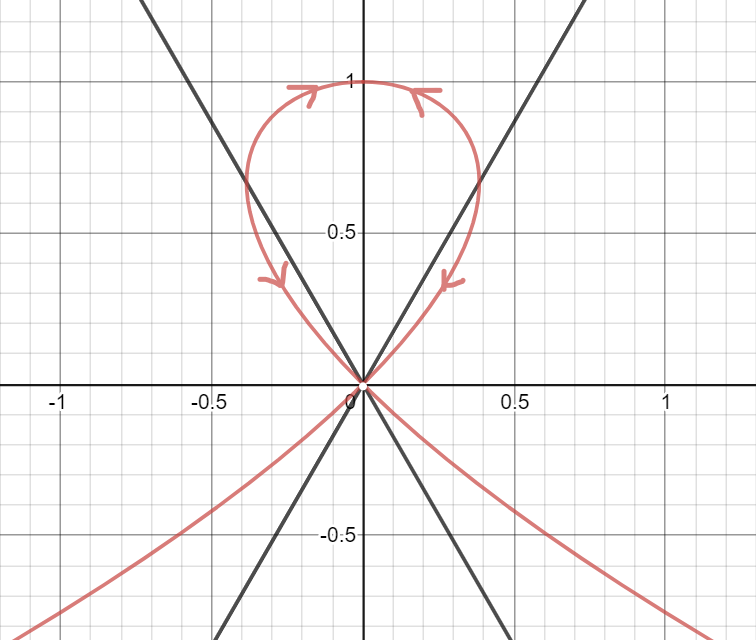
\includegraphics[scale=0.48]{graph4.1.png}} 
\end{center}
\[ y \rightarrow2/3 = \overline{y}\]
\[ 3\overline{x}^2 = \overline{y}^2\]
\textit{Домашнее задание:} найти решение для начальных условий $y(x_0) = y_0$\\

\chapter[{Семинар №5}]{Семинар №5}
\markright{Дифференциальные уравнения. Семинар № 5}
\thispagestyle{empty}

\textbf{Задача 1.} Решить дифференциальное уравнение (Задача Коши): 
\newline
\begin{equation}
y' = \frac 1 {y-x^2}
\end{equation}\\
с начальным условием
\begin{equation}
y(x_0)=y_0
\end{equation}\\
\textbf{Решение:} \par

Рассмотрим только случай $y_0>x_0^2$, т.е. начальные данные находятся выше параболы $y=x^2$.

1. Область определения:\\
\[D = \{(x,y)\in \textbf{R} ^2 \backslash y = x^2\}\]

2. Правая часть (5.1) непрерывно дифференцируема на области определения, следовательно, липшицева, следовательно, есть единственность на D. Отсюда следует, что для условия $y_0>x_0^2$  должно выполняться $y>x^2$.

3. Монотонность:\\
на $y>x^2$ производная вположительна, функция возрастает.\\
Промежутки выпуклости:
\[ y'' = - \frac {y'-2x} {(y-x^2)^2} = - \frac {1-2xy+2x^3} {(y-x^2)^3}\]
$ y''>0$, когда $1-2xy-2x^3<0$
\begin{center}
{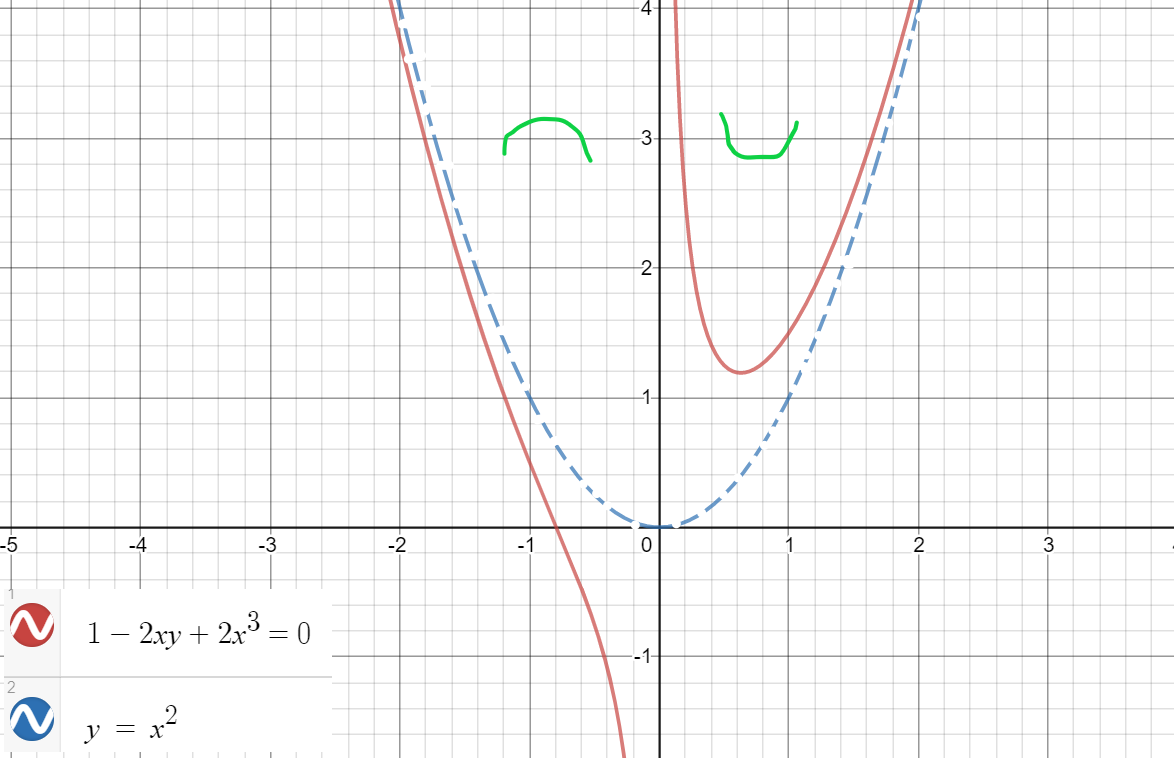
\includegraphics[scale=0.4]{graph5.1.png}} 
\end{center}

4. Максимальный интервал существования решения (a; b):

4.1. Рассмотрим правую границу b. Всего есть два возможных варианта:

а) Если b конечно ($ b \in \textbf{R}$):\\
a.I) b -- асимптота, а y неограничено растет: \[ \lim\limits_{x\to b-} y(x) = + \infty \]
подставляя в (5.1) $\Rightarrow$ 
\[ \lim\limits_{x\to b-} y'(x) = 0\]
В таком случае, у нашего решения есть асимптота b, y стремится на бесконечность с нулевой производной. Из геометрических соображений очевидно, что этот случай невозможен. Докажем это. Предположим, что такой случай все-таки возможен. Производная ограничена какой-то константой: 
\[|y'(x)| \leq C, \forall x >  \overline {x}\]
\[y' (x) \leq C\]
Обозначим:
\[y(\overline{x}) = \overline{y}\]
Сравним этот случай со следующим:
\begin{equation}
z' (x) = C
\end{equation}
\begin{equation}
z(\overline{x}) = \overline{y}
\end{equation}
 интегрируя (5.3) с учетом (5.4), получим, что 
\[ z(x) = C(x-\overline{x})+\overline{y}\]
отсюда следует неравенство
\[ y(x) \leq z(x) = C(x-\overline{x})+\overline{y}\] при $ x \geq \overline{x}$.
Получили, что y(x), стремящаяся к бесконечности, начиная с  $\overline{x}$ находится не выше линейной функции. Однако линейная функция должна пересечь параболу в точке с конечными координатами. Пришли к противоречию.\\ 
a.II) Следующий случай -- b конечно, а траектория утыкается в параболу, т.е.:
\[ \lim\limits_{x\to b-} y(x) = b^2\]
\[\lim\limits_{x\to b-} y'(x) = \frac {1} {b^2-b^2} = +\infty\]
-- этот случай также невозможен из геометрических соображений. Докажем это более строго.
\[y(x) \geq x^2\]
\[y(x)-b^2 \geq x^2-b^2\]
т.к. $x<b$:
\[ \frac {y(x)-b^2} { x-b} \leq  \frac {x^2-b^2} { x-b} = x+b\]
\[ \lim\limits_{x\to b-} \frac {y(x)-b^2} { x-b} \leq \lim\limits_{x\to b-} (x+b) = 2b\]
Применяя правило Лопиталя:
\[ \lim\limits_{x\to b-} \frac {y(x)-b^2} { x-b}  =\lim\limits_{x\to b-} y'(x)\]
Выходит, что производная $y'(x)$ не превосходит $2b$. Выходит, что и этот случай невозможен. Тогда остается только 1 возможный вариант для значения b:

b) $ b = +\infty$\\

4.2. Далее рассмотрим левую границу $a$.  Т.к. функция монотонно возрастает, то случай a) $ a = -\infty$ невозможен.\\
b) $a \in \textbf {R}$\\
Кроме того, y(x) не может устремиться к $-\infty$, тогда решение обязательно должно закончится на параболе:
\[\lim\limits_{x\to a+} y(x) =a^{+}\]
найдем производную, с которой решение входит в параболу:
\[\lim\limits_{x\to a+} y'(x) =\lim\limits_{x\to a+} \frac 1 {a^2-a^2} =+\infty\]

5. Поведение функции при $x\to +\infty$:\\
Предположим, что
\[ \lim\limits_{x\to +\infty} y(x) = x^2+O(1)\] -- докажем это по определению предела. Попробуем опровергнуть это.
\[ \lim\limits_{x\to 0} y(x) - x^2 =0  \; \Leftrightarrow \; \forall \varepsilon >0 \: \exists \: \overline{x}, \; \forall x > \overline{x}: \, |y-x^2|<\varepsilon\] 
Построим отрицание к существованию предела:\\
\[\exists C >0 \: \forall  \: \overline{x}, \; \exists  x > \overline{x}: |y(x_k) - x_k^2| \geq C\]
Тогда мы можем построить такую последовательность, что для $x_k \rightarrow +\infty $  выполняется $y(x_k) - x_k^2\geq C$
\[ y'(x_k) = \frac 1 {y(x_k) - x_k^2} \leq \frac 1 C\]
Значит, начиная  с $x_k$ производная ограничена.
\[y(x) \leq \frac 1 C (x-x_0) + y(x_0)\]
Рассматривая правую границу максимального интервала существования решения, мы доказали, что этот случай невозможен. Противоречие. Следовательно, $ \lim\limits_{x\to +\infty} y(x) = x^2+O(1)$.\\
Графическое решение уравнения (5.1) для случая $y_0>x_0^2$\\
\begin{center}
{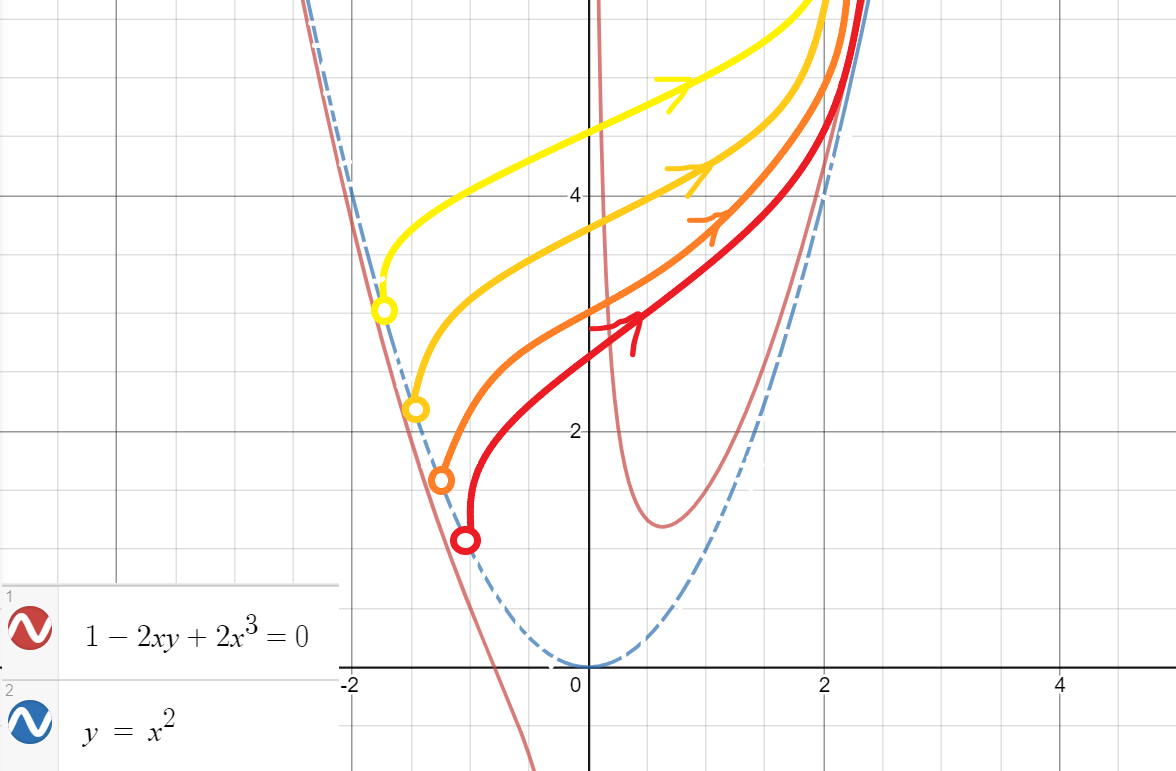
\includegraphics[scale=0.4]{graph5.2.png}} 
\end{center}
\textit{Домашнее задание: решить задачу для случая $y_0<x_0^2$}\\

\textbf{Задача 2.} Решить дифференциальное уравнение (Задача Коши): 
\newline
\begin{equation}
y' = |y| - x^2
\end{equation}\\
с начальным условием
\begin{equation}
y(0)=0
\end{equation}\\
\textbf{Решение:} \par
1. D = \{$\textbf{R}^2$\}

2. Модуль -- липшицева функция (хотя и не является дифференцируемой), следовательно, решение единственно на D.

3. Раскроем модуль:\\
при $y>0$ $ y'(x) = y-x^2$\\
при $y\leq 0$ $y'(x)=-y-x^2$

4. Симметрия:\\
$ u(x) = -y(-x)$\\
$u'(x) = y(-x) = |y(-x)|-x^2=|u(x)|-x^2$
Т.к. рассматриваем траекторию, проходящую через $(0;0),$ достаточно рассматривать y на одном из промежутков $y>0$ или $y\leq 0$, а затем симметрично отразить относительно начала координат.

5. Сравним два случая:\\
I. \[y' \leq |y|\]
\[y(0)=0\]
\[x>0\]
II.  \[z' = |z|\]
\[z(0)=0\]
\[x>0\]
В каждой точке производная второй функции больше, чем производная первой, поэтому при $x>0$ $y(x) \leq z(x)$. Стационарное решение II $z(x)=0$. Для уравнения II существует единственность (снова, модуль -- липщицева функция). Поэтому  $z(x)=0$ единственное решение с заданными начальными данными. Тогда 
y(x) -- отрицательно для $x>0$. Все аналогично для случая $x\leq 0$.

6. Рассмотрим \[y'=-y-x^2\]
Для случая $y>0$ найдем решение линейного дифференциального уравнения как сумму частного и общего решений. Справа стоит $x^2$, поэтому ищем решение в виде $y_{*}=ax^2+bx+c$. Подставим $y_{*}$:\\
\[2ax+b=ax^2+bx+c-x^2,\]
откуда $a=1 \; b=2, \; c = 2$. 
Найдем общее решение $y_{hom}' = y_{hom}, $\\$ y_{hom}=e^{x}$.\\
Тогда общее решение:
\[ y(x) = Ce^{x}+x^2+2x+2, \; y\leq 0\]
Аналогично для случая $x>0$
\[ y(x) = Ce^{-x}-x^2+2x-2, \; y>0\]
С учетом начальных данных:
\[ y(x) = 2e^{-x}-x^2+2x-2, \; y>0\]
\[ y(x) = -2e^{x}+x^2+2x+2, \; y\leq 0\]
\begin{center}
{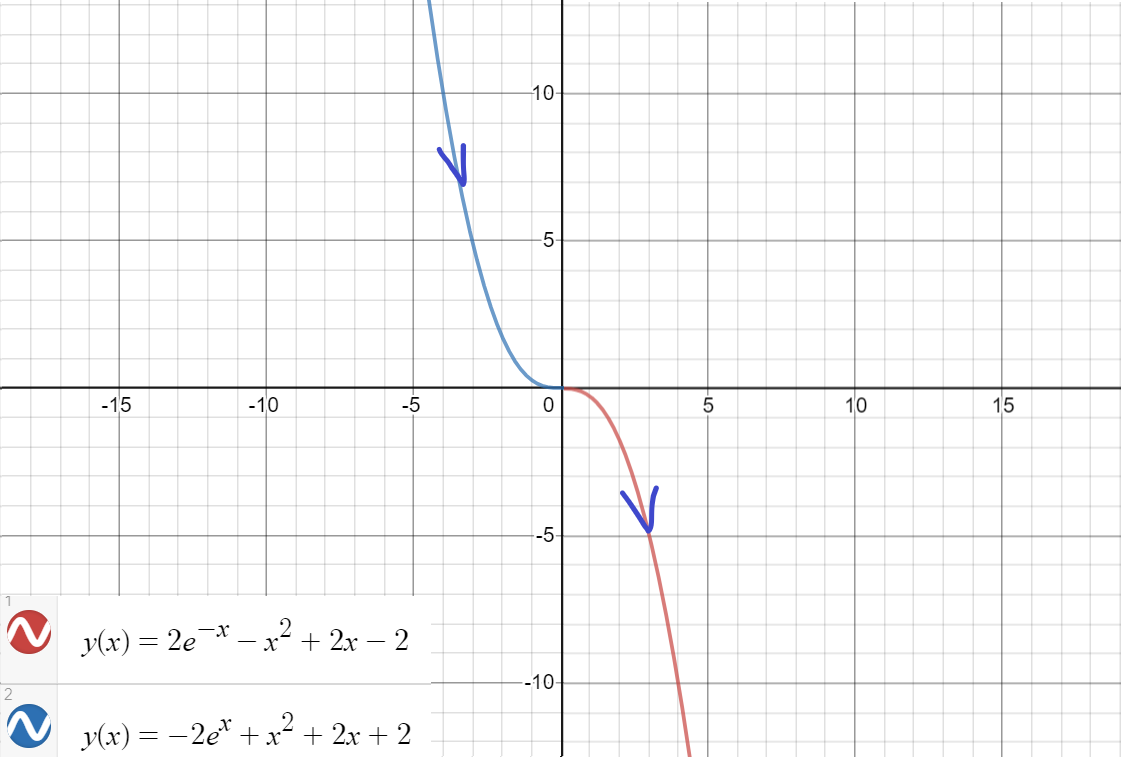
\includegraphics[scale=0.4]{graph5.3.png}} 
\end{center}
\textit{Домашнее задание: решить задачу для начальных данных $y(x_0) = y_0$}

\chapter[{Семинар: консультация перед контрольной работой №1}]{Семинар: консультация перед контрольной работой №1}
\markright{Консультация перед контрольной работой №1}
\thispagestyle{empty}
\maketitle
\textbf{Задача 1.} Решить дифференциальное уравнение (Задача Коши): 
\newline
\begin{equation}
\dot {x} = \frac {t+x-3} {t-x-1}
\end{equation}\\
с начальным условием
\begin{equation}
x(t_0) = x_0
\end{equation}\\
\textbf{Решение:} \par
Для начала сделаем замену:\\
\[y=t-2\]
\[z=x-1\]
тогда
\[\dot{z} = \dot {x}\]
(6.1) преобразуется в\\
\[ \dot{z}= \frac {y+z} {y-z}\]
Такой заменой мы свели задачу к задаче 1 семинара №3. Чтобы получить решение этого уравнения, нужно перенести центр (0; 0) системы координат Ozy в точку (1; 2) системы координат Oxt:
\begin{center}
{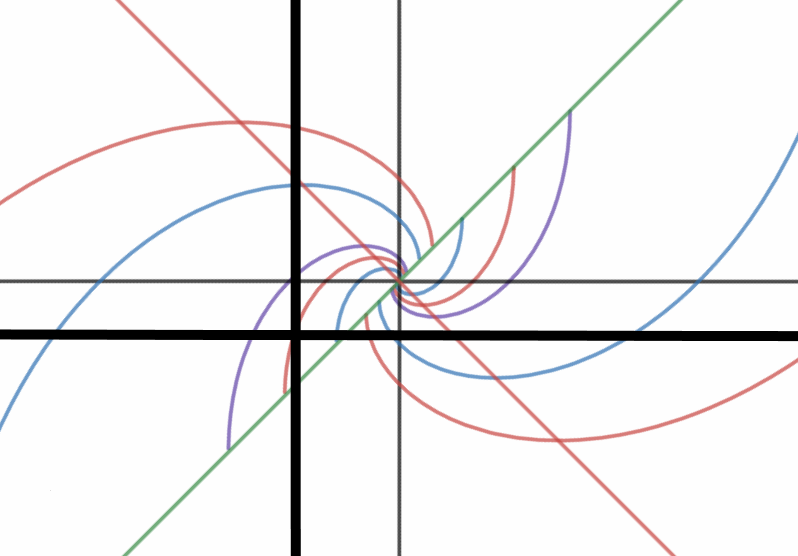
\includegraphics[scale=0.5]{graph6.1.png}} 
\end{center}
\maketitle
\textbf{Задача 2.} Решить дифференциальное уравнение (Задача Коши): 
\newline
\begin{equation}
\dot {x}(x+1) = \frac {x} {1+t^2}
\end{equation}\\
с начальным условием
\begin{equation}
x(t_0) = x_0
\end{equation}\\
\textbf{Решение:} \par
1) Чтобы применить теоремы о существовании и единственности решения, нужно привести уравнение (6.3) к виду 
\begin{equation}
\dot {x} = \frac {x} {(1+t^2)(x+1)}
\end{equation}

Для этого отдельно рассмотрим случай $x=-1$. Левая часть (6.3) обращается в 0, а правая никогда не обращается в 0, следовательно, $(6.3) \Leftrightarrow (6.5)$.

2) $D: \{(t,x) \in \textbf{R}^2 \backslash x = 1\}$

3) По теореме Пеано решение локально существует, правая часть дифференцируема на D, следовательно, решения не пересекаются. 

4) Найдем промежутки возрастания:
\[\frac x {1+x} > 0\]
\begin{center}
{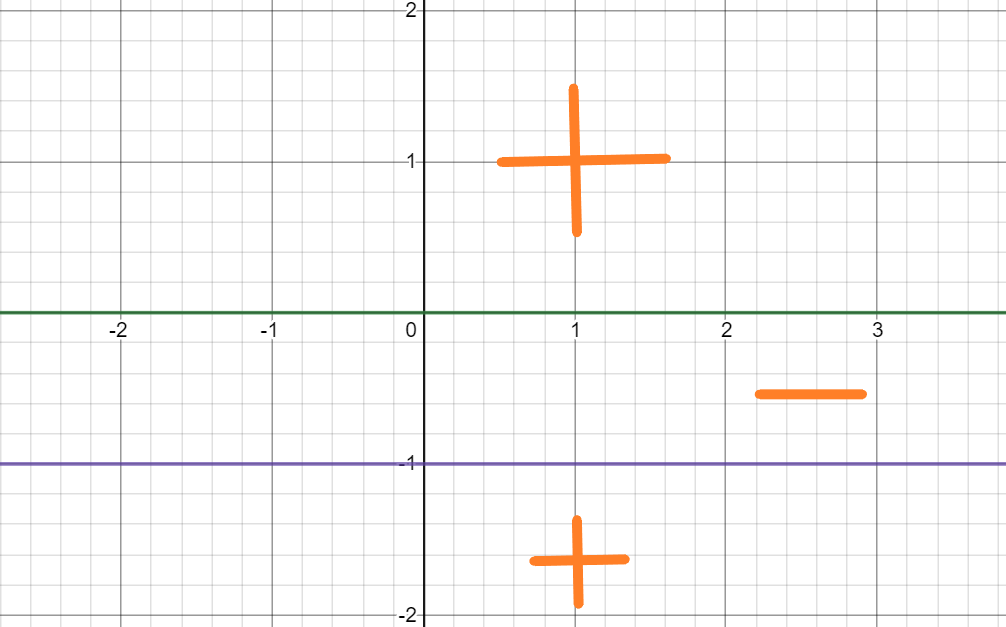
\includegraphics[scale=0.4]{graph6.2.png}} 
\end{center}

5) Стационарное решение: $x = const, x = 0$. Решим явно методом разделения переменных (6.5):
\[ (1+1/x)dx=\frac {dt} {1+t^2}\]
\begin{equation}
x+ln|x| = arctg(t)-arctg(t_0)+x_0+ln|x_0|
\end{equation}
Пусть $f(x) = x+ln|x|$. Построим f(x) 
\begin{center}
{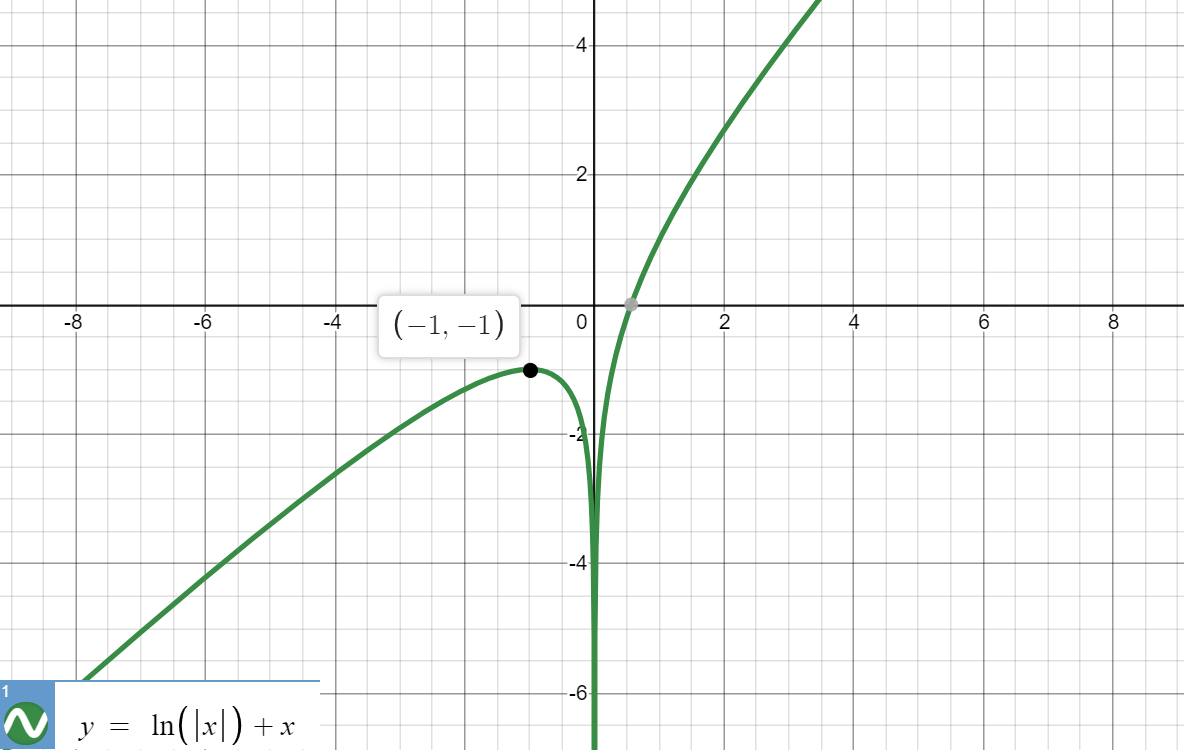
\includegraphics[scale=0.4]{graph6.3.png}} 
\end{center}
7) Правая часть (6.6) ограничена. Обозначим $C  = -arctg(t_0)+x_0+ln|x_0|$. Т.к. $arctg(t) \in(-\pi/2; \pi/2)$, то правая часть определена на $(C-\pi/2; C+\pi/2). $

a) $x \in (0; +\infty)$
Интервал существования -- все t. У каждой траектории есть своя асимптота, т.к. правая часть (6.6) ограничена. Производная положительна, все кривые возрастают. Для более точного построения кривых необходимо найти вторую производную и промежутки выпуклости.
\textit{Упражнение: найти промежутки выпуклости функции.}

b) $x \in (-1; 0)$
\[ f(x) \in (-1; -\infty)\]
Здесь необходимо рассмотреть 2 случая:\\
(i) Если $ \frac \pi 2 + C < -1 $ -- решение определено для всех t. Асимптоты справа и слева\\
(ii) Если   $ \frac \pi 2 + C > -1 $ -- решение существует на $ t \in (-\infty; \overline{t})$.  Асимптоты слева

c)   $x \in (-1; 0)$
\[ f(x) \in (-1; -\infty)\]
Аналогично, здесь необходимо рассмотреть 2 случая:\\
(i) Если $ \frac \pi 2 + C < -1 $ -- решение определено для всех t. У решений есть асимптоты справа и слева\\
(ii) Если   $ \frac \pi 2 + C > -1 $ -- решение существует на $ t \in (-\infty; \overline{t})$. Асимптоты слева\\
Изобразим сепаратрису случаев (i) и (ii):
\[ \frac \pi 2 + x_0 +ln|x_0| - arctg(t_0) = -1 \]
\begin{center}
{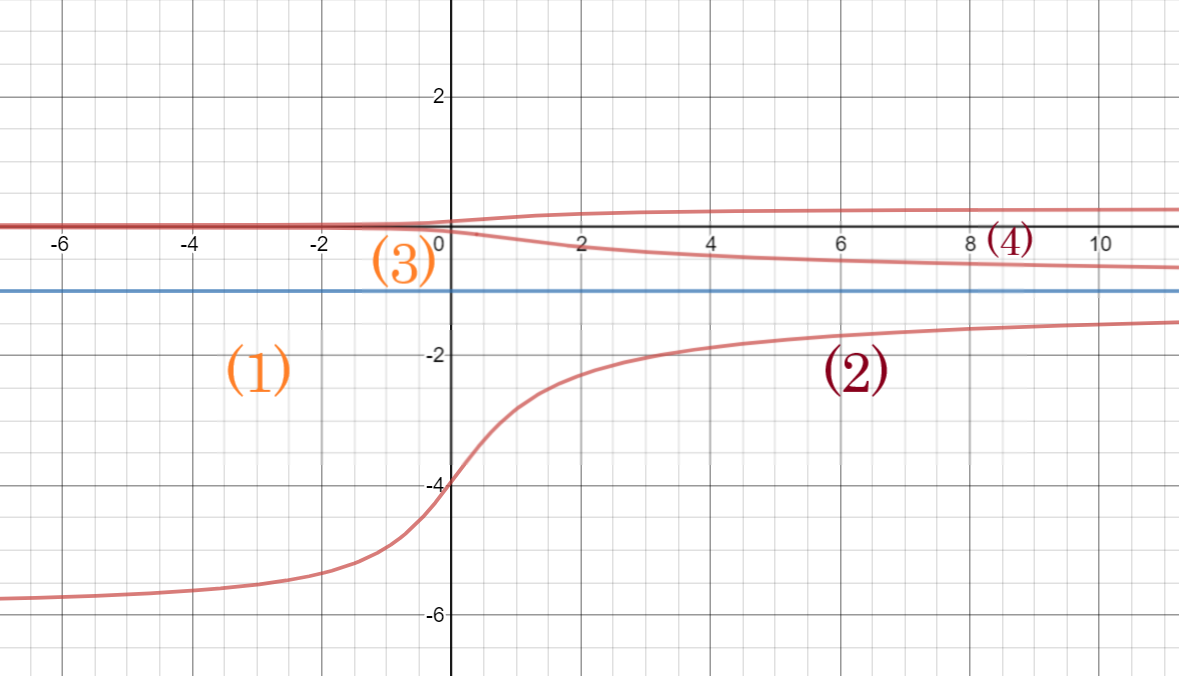
\includegraphics[scale=0.4]{graph6.4.png}} 
\end{center}
На графике области (1) и (3) соответствуют случаям b(i) и c(i), а области (2) и (4) -- b(ii) и c(ii).

8) Изобразим решения (6.3):
\begin{center}
{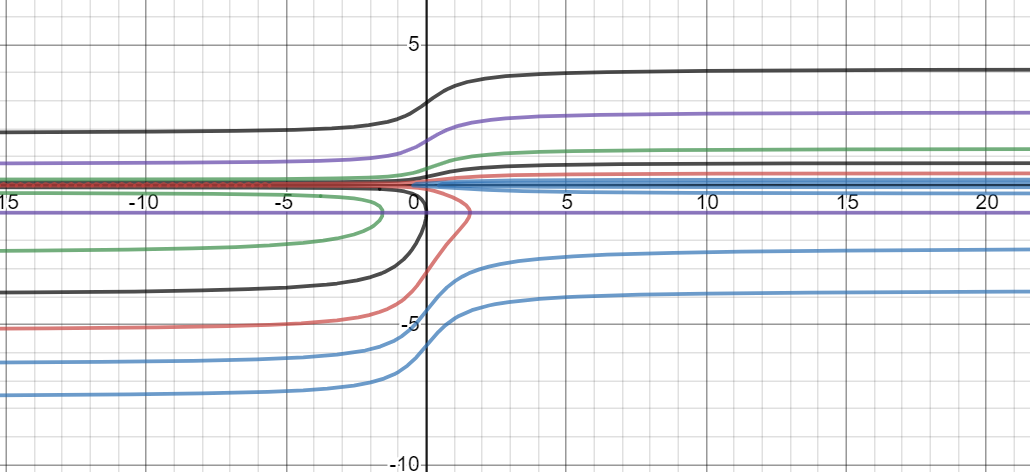
\includegraphics[scale=0.55]{graph6.5.png}} 
\end{center}

\markright{Дифференциальные уравнения. Семинар № 6}
\chapter[{Семинар №6}]{Семинар №6}
\thispagestyle{empty}
\section {Линейные системы}
\textbf{Задача 1.} Решить систему дифференциальных уравнений (Задача Коши): 
\begin{equation}
\left\{
\begin{array}{lr}
\dot{x} = 4x-2y\\
\dot{y} = 3x-3y
\end{array}
\right.
\end{equation}
с начальными условиями
\[ x(t_0)=x_0\]
\[y(t_0)=y_0\]
\textbf{Решение:} \par

Приведем (7.1) к виду
\begin{equation}
\left(
\begin{array}{c}
\dot{x}\\
\dot{y}\\
\end{array}
\right)
 = \left(
\begin{array}{cc}
4 & -2\\
3 & -3\\
\end{array}
\right)
\left(
\begin{array}{cc}
x\\
y\\
\end{array}
\right)
\end{equation}
Обозначим 
\[
A = \left(
\begin{array}{cc}
4 & -2\\
3 & -3\\
\end{array}
\right)\]

1. Найдем собственные числа матрицы A:
\[det(A-\lambda \hat{I})=
\begin{vmatrix}
4-\lambda & -2 \\
3 & -3-\lambda
\end{vmatrix}
=(4-\lambda)(-3-\lambda)+6=0\]
\[\lambda_1=-2, \; \lambda_2=3\]

2.  $\lambda_{1,2}$ разных знаков, картина -- седловая точка, 0 не является устойчивым решением.

3. Найдем собственные векторы A: Ap=$\lambda$p

3.1. $\lambda_1=-2$\\
\[(A-\lambda_1 \hat{I})p=0\]
\[\left(
\begin{array}{cc}
4+2 & -2\\
3 & -3+2
\end{array}
\right)
\left(
\begin{array}{cc}
p_1\\
p_2\\
\end{array}
\right)=
\left(
\begin{array}{c}
0\\
0
\end{array}
\right)
\]
Отсюда
\[p^1=
\left(
\begin{array}{cc}
1\\
3\\
\end{array}
\right)
\]

3.2. $\lambda_2=3$\\
\[(A-\lambda_2 \hat{I})p=0\]
\[\left(
\begin{array}{cc}
4-3 & -2\\
3 & -3-3
\end{array}
\right)
\left(
\begin{array}{cc}
p_1\\
p_2\\
\end{array}
\right)=
\left(
\begin{array}{c}
0\\
0
\end{array}
\right)
\]
Отсюда
\[p^2=
\left(
\begin{array}{cc}
2\\
1\\
\end{array}
\right)
\]

4. Тогда общее решение уравнения (7.1):
\begin{equation}
\left(
\begin{array}{c}
x(t)\\
y(t)
\end{array}
\right)
=C_1p^1e^{\lambda_1(t-t_0)}+C_1p^2e^{\lambda_2(t-t_0)}
\end{equation}
\[\left(
\begin{array}{c}
x(t)\\
y(t)
\end{array}
\right)
=C_1
\left(
\begin{array}{c}
1\\
3
\end{array}
\right)
e^{-2(t-t_0)}+C_2
\left(
\begin{array}{c}
2\\
1
\end{array}
\right)
e^{3(t-t_0)}
\]
Найдем константы из начальных условий:
\[\left(
\begin{array}{c}
x_0\\
y_0
\end{array}
\right)
=C_1
\left(
\begin{array}{c}
1\\
3
\end{array}
\right)+C_2
\left(
\begin{array}{c}
2\\
1
\end{array}
\right)
\]
\[
\left(
\begin{array}{c}
x_0\\
y_0\\
\end{array}
\right)
 = \left(
\begin{array}{cc}
1 & 2\\
3 & 1\\
\end{array}
\right)
\left(
\begin{array}{cc}
C_1\\
C_2\\
\end{array}
\right)
\]
\[ T= \left(
\begin{array}{cc}
1 & 2\\
3 & 1
\end{array}
\right)\]
Найдем обратную матрицу к T:
\[T^{-1}  = \left(
\begin{array}{cc}
-1/5 & 2/5\\
3/5 & -1/5
\end{array}
\right)\]
\[
\left(
\begin{array}{c}
C_1\\
C_2\\
\end{array}
\right)
 = \left(
\begin{array}{cc}
-1/5 & 2/5\\
3/5 & -1/5
\end{array}
\right)
\left(
\begin{array}{cc}
x_0\\
y_0\\
\end{array}
\right)
\]
Тогда решение (7.1):
\[\left(
\begin{array}{c}
x(t)\\
y(t)
\end{array}
\right)
=(-1/5x_{0}+2/5y_{0})
\left(
\begin{array}{c}
1\\
3
\end{array}
\right)
e^{-2(t-t_0)}+(3/5x_{0}-1/5y_{0})
\left(
\begin{array}{c}
2\\
1
\end{array}
\right)
e^{3(t-t_0)}
\]

5. Рассмотрим выражение (7.3). Если $C_1$ или $C_2$ -- все решения продолжаются по прямой, задаваемой одним из собственных векторов. Направление траекторий определяется знаком $\lambda$: в случае $\lambda_1=-2$ при $ t \rightarrow +\infty \;\;\;  x(t), y(t) \Rightarrow 0$, $\lambda_2=3$ при $ t \rightarrow +\infty \;\;\;  x(t), y(t) \Rightarrow +\infty$, а для $ t \rightarrow -\infty$ в обоих случаях все аналогично. Устойчивости нет. \\
При $ t \rightarrow +\infty$ в случае $C_1, C_2 \neq 0 $ все траектории стремятся к $y= \frac x 2$, а при $ t \rightarrow - \infty$ --- к $y= 3x.$
\begin{center}
{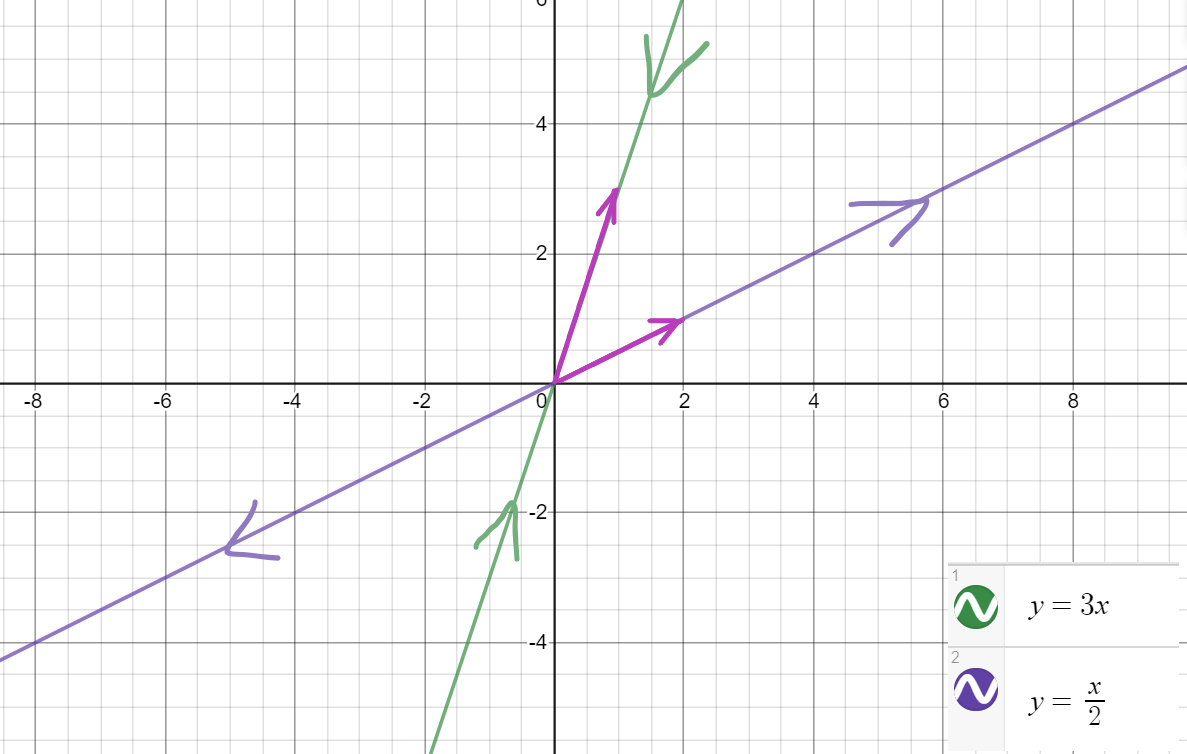
\includegraphics[scale=0.4]{graph7.4.png}} 
\end{center}

6. Найдем нули производных и отметим их на фазовом портрете. Эти прямые решения пересекают с нулевой производной. \[ \dot{x}=0 \Leftrightarrow y=2x\]
\[ \dot{y}=0 \Leftrightarrow y=x\]
\begin{center}
{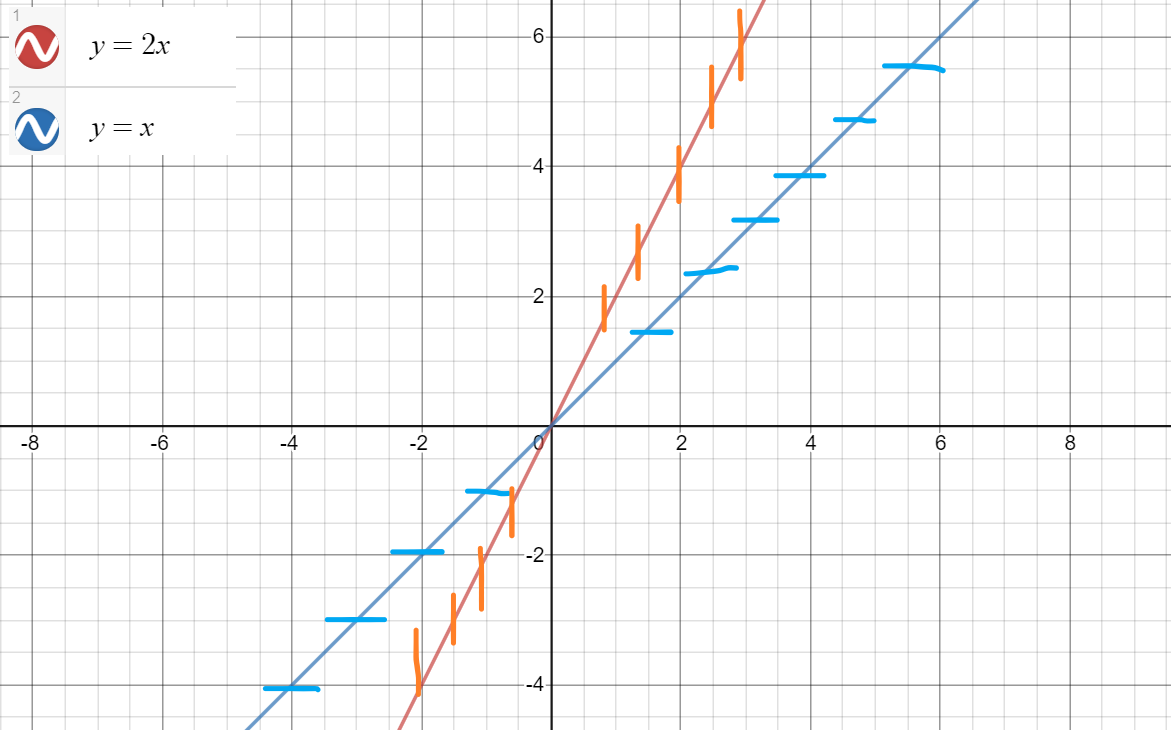
\includegraphics[scale=0.4]{graph7.3.png}} 
\end{center}

7. Изобразим общую картину траекторий:
\begin{center}
{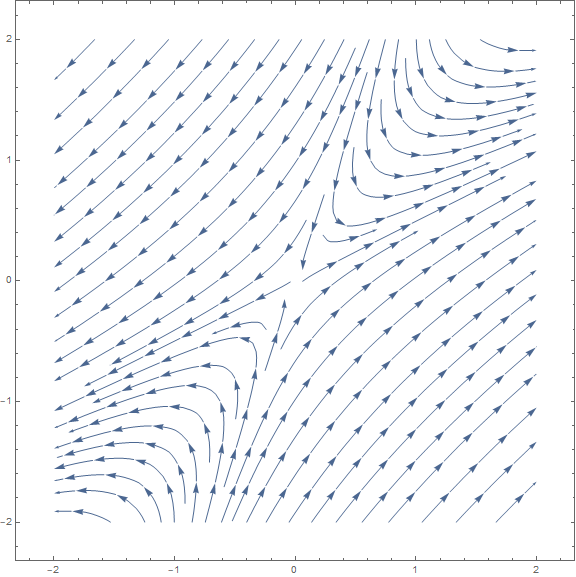
\includegraphics[scale=0.5]{graph7.2.png}} 
\end{center}
\textbf{Задача 2.} Решить систему дифференциальных уравнений (Задача Коши): 
\begin{equation}
\left\{
\begin{array}{lr}
\dot{x} = 4x+2y\\
\dot{y} = x+3y
\end{array}
\right.
\end{equation}
с начальными условиями
\[ x(t_0)=x_0\]
\[y(t_0)=y_0\]
\textbf{Решение:} \par
Обозначим 
\[
A = \left(
\begin{array}{cc}
4 & 2\\
1 & 3\\
\end{array}
\right)\]
1. Найдем собственные числа матрицы A:
\[det(A-\lambda \hat{I})=
\begin{vmatrix}
4-\lambda & 2 \\
1 & 3-\lambda
\end{vmatrix}
=(4-\lambda)(3-\lambda)-2=0\]
\[\lambda_1=2, \; \lambda_2=5\]
2.  $\lambda_{1,2}$ больше 0, картина -- неустойчивый узел.

3. Найдем собственные векторы A: Ap=$\lambda$p

3.1. $\lambda_1=2$\\
\[(A-\lambda_1 \hat{I})p=0\]
\[\left(
\begin{array}{cc}
4-2 & 2\\
1 & 3-2
\end{array}
\right)
\left(
\begin{array}{cc}
p_1\\
p_2\\
\end{array}
\right)=
\left(
\begin{array}{c}
0\\
0
\end{array}
\right)
\]
Отсюда
\[p^1=
\left(
\begin{array}{cc}
-1\\
1\\
\end{array}
\right)
\]

3.2. $\lambda_2=5$\\
\[(A-\lambda_1 \hat{I})p=0\]
\[\left(
\begin{array}{cc}
4-5 & 2\\
1 & 3-5
\end{array}
\right)
\left(
\begin{array}{cc}
p_1\\
p_2\\
\end{array}
\right)=
\left(
\begin{array}{c}
0\\
0
\end{array}
\right)
\]
Отсюда
\[p^2=
\left(
\begin{array}{cc}
2\\
1\\
\end{array}
\right)
\]

4. Тогда общее решение уравнения (7.4):
\[\left(
\begin{array}{c}
x(t)\\
y(t)
\end{array}
\right)
=C_1
\left(
\begin{array}{c}
-1\\
1
\end{array}
\right)
e^{2(t-t_0)}+C_2
\left(
\begin{array}{c}
2\\
1
\end{array}
\right)
e^{5(t-t_0)}
\]
Найдем константы из начальных условий:
\[\left(
\begin{array}{c}
x_0\\
y_0
\end{array}
\right)
=C_1
\left(
\begin{array}{c}
-1\\
1
\end{array}
\right)+C_2
\left(
\begin{array}{c}
2\\
1
\end{array}
\right)
\]
\[
\left(
\begin{array}{c}
x_0\\
y_0\\
\end{array}
\right)
 = \left(
\begin{array}{cc}
-1 & 2\\
1 & 1\\
\end{array}
\right)
\left(
\begin{array}{cc}
C_1\\
C_2\\
\end{array}
\right)
\]
\[ T= \left(
\begin{array}{cc}
-1 & 2\\
1 & 1
\end{array}
\right)\]
Найдем обратную матрицу к T:
\[T^{-1}  = \left(
\begin{array}{cc}
-1/3 & 2/3\\
1/3 & 1/3
\end{array}
\right)\]
\[
\left(
\begin{array}{c}
C_1\\
C_2\\
\end{array}
\right)
 = \left(
\begin{array}{cc}
-1/3 & 2/3\\
1/3 & 1/3
\end{array}
\right)
\left(
\begin{array}{cc}
x_0\\
y_0\\
\end{array}
\right)
\]
Тогда решение (7.4):
\[\left(
\begin{array}{c}
x(t)\\
y(t)
\end{array}
\right)
=(-1/3x_{0}+2/3y_{0})
\left(
\begin{array}{c}
-1\\
1
\end{array}
\right)
e^{2(t-t_0)}+(1/3x_{0}+1/3y_{0})
\left(
\begin{array}{c}
2\\
1
\end{array}
\right)
e^{5(t-t_0)}
\]

5. Изобразим собственные вектора и соответствующие им прямые. Т.к. оба собственных значения больше нуля -- решения уходят от нуля на бесконечность при $t \rightarrow +\infty$
\begin{center}
{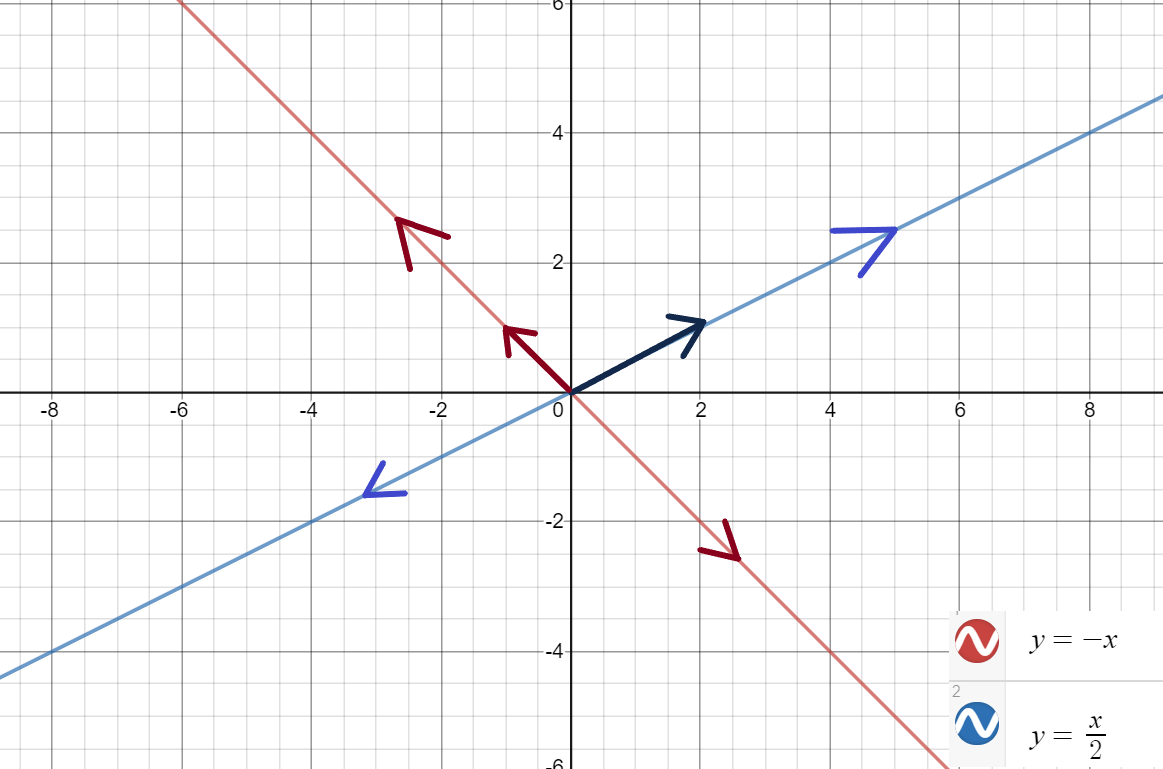
\includegraphics[scale=0.4]{graph7.5.png}} 
\end{center}

6. Найдем нули производных и отметим их на фазовом портрете\[ \dot{x}=0 \Leftrightarrow y=-2x\]
\[ \dot{y}=0 \Leftrightarrow -3y=x\]
\begin{center}
{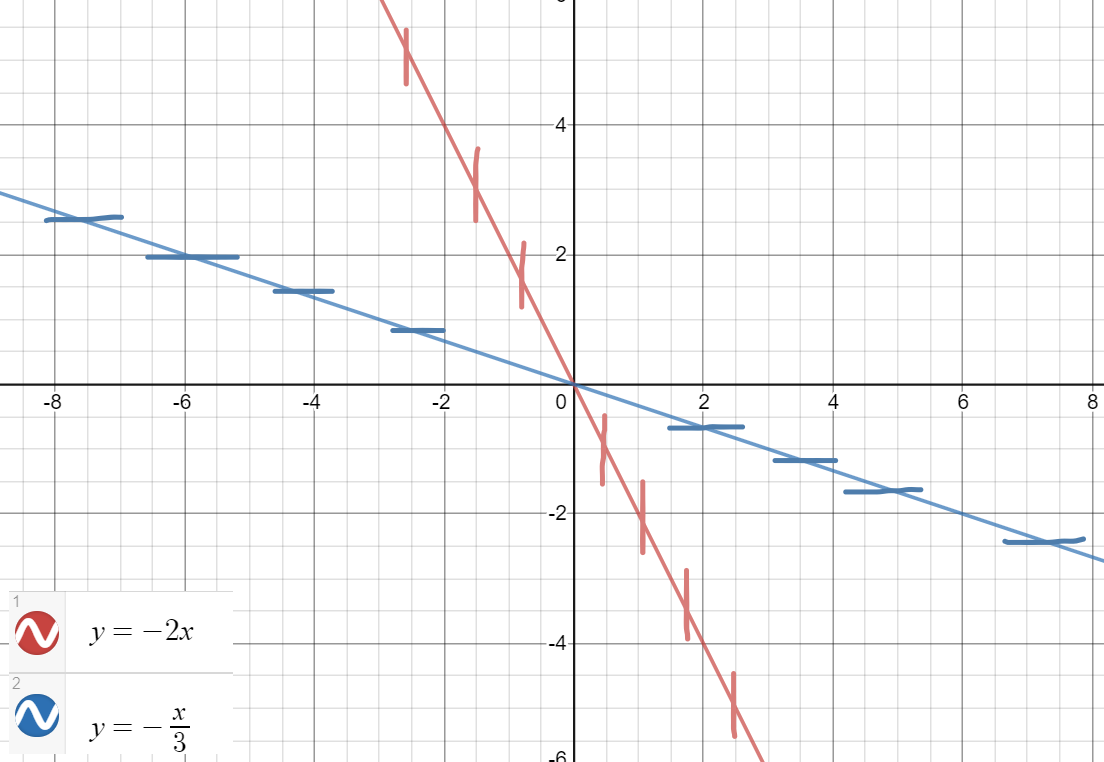
\includegraphics[scale=0.4]{graph7.6.png}} 
\end{center}

7. Изобразим общую картину траекторий:
\begin{center}
{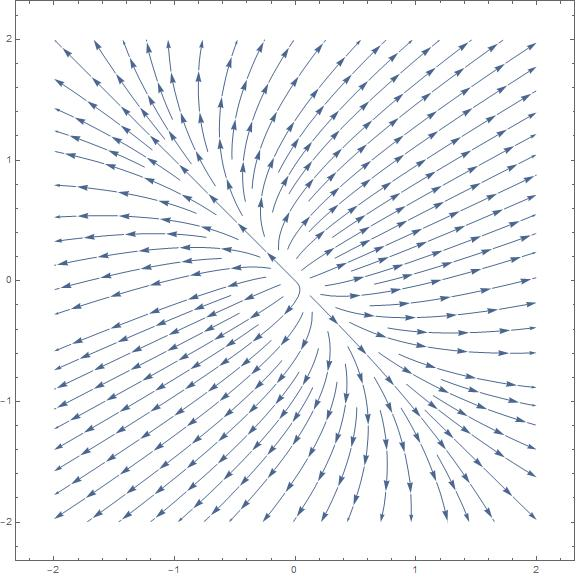
\includegraphics[scale=0.5]{graph7.1.jpg}} 
\end{center}

\textit{Домашнее задание:\\
$\dot{x}=x/2-y$\\
$\dot{y}=x-y$}

\markright{Дифференциальные уравнения. Семинар № 7}
\chapter[{Семинар №7}]{Семинар №7}
\thispagestyle{empty}
\textbf{Задача 1.} Решить систему дифференциальных уравнений (Задача Коши): 
\begin{equation}
\left\{
\begin{array}{lr}
\dot{x} = -6x-5y\\
\dot{y} = 5x+4y
\end{array}
\right.
\end{equation}
с начальными условиями
\[ x(t_0)=x_0\]
\[y(t_0)=y_0\]\\
\textbf{Решение:} \par
Обозначим 
\[
A = \left(
\begin{array}{cc}
-6 & -5\\
5 & 4\\
\end{array}
\right)\]

1. Найдем собственные числа матрицы A:
\[det(A-\lambda \hat{I})=
\begin{vmatrix}
-6-\lambda & -5 \\
5 & 4-\lambda
\end{vmatrix}
=(-6-\lambda)(4-\lambda)+25=0\]
\[\lambda =-1\]
Получили собственное число кратности 2.

2.  Найдем собственный вектор:
\[(A-\lambda \hat{I})p=0\]
\[\left(
\begin{array}{cc}
-6+1 & -5\\
5 & 4+1
\end{array}
\right)
\left(
\begin{array}{cc}
p_1\\
p_2\\
\end{array}
\right)=
\left(
\begin{array}{c}
0\\
0
\end{array}
\right)
\]
Отсюда
\[p^1=
\left(
\begin{array}{cc}
-1\\
1\\
\end{array}
\right)
\]
Причем пространство векторов имеет размерность 1:
\[dim \{ p\in \textbf {R}^2: p_1^1=-p_2^1\}=1\]
Собственному числу соответствует одномерное пространство собственных векторов. Найдем присоединенный вектор:\\
\[(A-\lambda \hat{I})v=p^1\]
\[\left(
\begin{array}{cc}
-6+1 & -5\\
5 & 4+1
\end{array}
\right)
\left(
\begin{array}{cc}
v_1\\
v_2\\
\end{array}
\right)=
\left(
\begin{array}{c}
-1\\
1
\end{array}
\right)
\]
Отсюда
\[v^2=
\left(
\begin{array}{cc}
1/5\\
0\\
\end{array}
\right)
\]

3. Тогда общее решение уравнения (8.1) согласно теории из лекции:
\[
\left(
\begin{array}{c}
x(t)\\
y(t)
\end{array}
\right)
=C_1
\left(
\begin{array}{c}
-1\\
1
\end{array}
\right)
e^{-t}+C_2
\left(
te^{-t}
\left(
\begin{array}{c}
-1\\
1
\end{array}
\right)
+e^{-t}
\left(
\begin{array}{c}
1/5\\
0
\end{array}
\right)
\right)
\]
\textit{Домашнее задание: найти $C_1$ и $C_2$}\\

4. Найдем нули производных и отметим их на фазовом портрете. Эти прямые решения пересекают с нулевой производной. \[ \dot{x}=0 \Leftrightarrow y=-6/5x\]
\[ \dot{y}=0 \Leftrightarrow y=-5/4x\]
Рисунок -- устойчивый вырожденный узел.
\begin{center}
{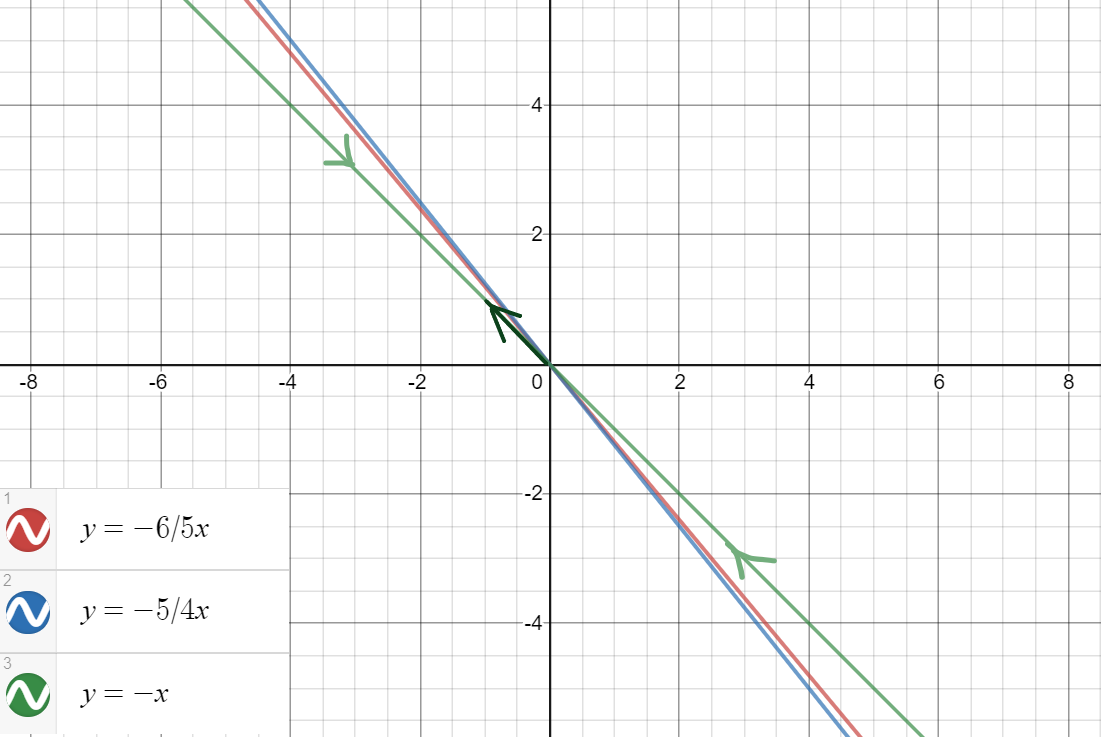
\includegraphics[scale=0.4]{graph8.1.png}} 
\end{center}

5. Изобразим общую картину траекторий:

\begin{center}
{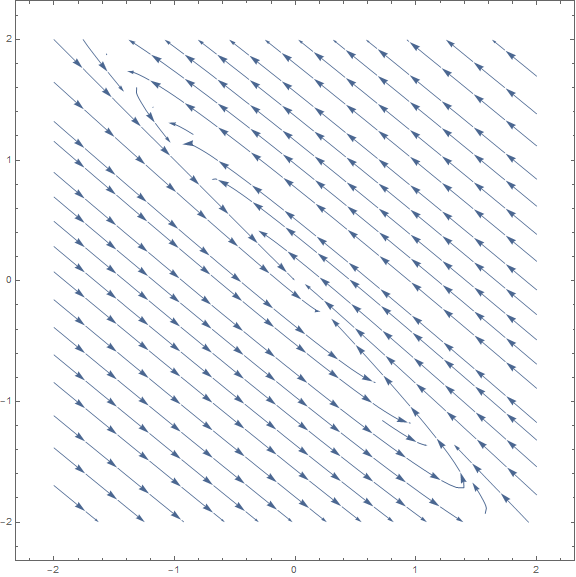
\includegraphics[scale=0.5]{graph8.2.png}} 
\end{center}

\section {Метод вариации произвольных постоянных}
\textbf{Задача 2.} Решить систему дифференциальных уравнений: 
\begin{equation}
\left\{
\begin{array}{lr}
\dot{x} = 2x-y+e^{2t}\\
\dot{y} = 6x-3y+e^t+1
\end{array}
\right.
\end{equation}\\
\textbf{Решение:} \par
Обозначим 
\[
A = \left(
\begin{array}{cc}
2 & -1\\
6 & -3\\
\end{array}
\right)\]
Тогда
\[
\left(
\begin{array}{c}
\dot{x}\\
\dot{y}
\end{array}
\right)=
A
\left(
\begin{array}{c}
x\\
y
\end{array}
\right)
+
\left(
\begin{array}{c}
e^{2t}\\
1+e^t
\end{array}
\right)
\]

1. Найдем решение однородного уравнения
\[\left(
\begin{array}{c}
\dot{x}\\
\dot{y}
\end{array}
\right)=
A
\left(
\begin{array}{c}
x\\
y
\end{array}
\right)\]
Собственные числа матрицы A:
\[det(A-\lambda \hat{I})=
\begin{vmatrix}
2-\lambda & -1 \\
6 & -3-\lambda
\end{vmatrix}
=(2-\lambda)(-3-\lambda)+6=0\]
\[\lambda_1 =0, \; \; \lambda_1 =-1\]
Собственные вектора:\\

а) Для $\lambda_1=0:$
\[v^1=
\left(
\begin{array}{c}
1\\
2
\end{array}
\right)
\]

б) Для $\lambda_2=-1:$
\[v^2=
\left(
\begin{array}{c}
1\\
3
\end{array}
\right)
\]
Тогда напишем общее решение однородного уравнения:
\[
\left(
\begin{array}{c}
x\\
y
\end{array}
\right)
= C_1
\left(
\begin{array}{c}
1\\
2
\end{array}
\right)
+C_2e^{-t}
\left(
\begin{array}{c}
1\\
3
\end{array}
\right)
\]

2. Решим неоднородное уравнение:\\
Ищем решение в виде:
\[x := C_1(t)+C_2(t)e^{-t}\]
\[y := 2C_1(t)+3C_2(t)e^{-t}\]
Подставляя эти выражения в (8.2):
\begin{equation}
\dot{x} = \dot{C_1}+\dot{C_2}e^{-t}-C_2e^{-t}=2(C_1+C_2e^{-t})-2C_1-3C_2e^{-t}+e^{2t}
\end{equation}
\begin{equation}
\dot{y} = 2\dot{C_1}+3\dot{C_2}e^{-t}-3C_2e^{-t}=6(C_1+C_2e^{-t})-3(2C_1+3C_2e^{-t})+1+e^{t}
\end{equation}
Из (8.3) следует
\[ \dot{C_1}+\dot{C_2}e^{-t}=e^{2t}\]
Из (8.4) следует
\[ 2\dot{C_1}+3\dot{C_2}e^{-t}=1+e^{t}\]
Объединяя эти выражения:
\begin{equation}
\left(
\begin{array}{cc}
1 & e{-t}\\
2 & 3e^{-t}\\
\end{array}
\right)
\left(
\begin{array}{c}
\dot{C_1}\\
\dot{C_2}\\
\end{array}
\right)=
\left(
\begin{array}{c}
e^{2t}\\
1+e^{2t}\\
\end{array}
\right)
\end{equation}
Обозначим 
\[ B=
\left(
\begin{array}{cc}
1 & e{-t}\\
2 & 3e^{-t}\\
\end{array}
\right)\]
Найдем обратную матрицу к B:
\[ B^{-1}=
e^{t}\left(
\begin{array}{cc}
3 & -e^{-t}\\
-2 & 1\\
\end{array}
\right)\]
Тогда из (8.5):
\[
\left(
\begin{array}{c}
\dot{C_1}\\
\dot{C_2}\\
\end{array}
\right)=
e^{t}\left(
\begin{array}{cc}
3 & -e^{-t}\\
-2 & 1\\
\end{array}
\right)
\left(
\begin{array}{c}
e^{2t}\\
1+e^{2t}\\
\end{array}
\right)=
\left(
\begin{array}{c}
3e^{2t}-1-e^t\\
-2e^{3t}+e^t+e^{2t}
\end{array}
\right)
\]
Интегрируя, находим $C_1$ и $C_2$ находим константы для частного решения:
\[
\left(
\begin{array}{c}
C_1\\
C_2\\
\end{array}
\right)=
\left(
\begin{array}{c}
\frac 3 2 e^{2t}-t-e^t+C_{01}\\
-\frac 2 3e^{3t}+e^t+\frac {e^{2t}} 2 +C_{02}
\end{array}
\right)\]
Тогда решение имеет вид:
\[x = \frac 3 2 e^{2t}-t-e^t+C_{01}+\left( -\frac 2 3e^{3t}+e^t+\frac {e^{2t}} 2 +C_{02}\right)e^{-t}=-t+1+C_{01}+C_{02}e^{-t}-\frac 1 2 e^t+\frac 5 6e^{2t}\]
\[y =  3 e^{2t}-2t-2e^t+2C_{01}+\left( -2 e^{3t}+3e^t+\frac {3e^{2t}} 2 +3C_{02}\right)e^{-t}=e^{2t}-2t-\frac 1 2 e^t+2C_{01}+3+3C_{02}e^{-t}\]

\textbf{Задача 3.} Решить систему дифференциальных уравнений: 
\begin{equation}
\left\{
\begin{array}{lr}
\dot{x} = y+\frac 1 {cost}\\
\dot{y} = -x
\end{array}
\right.
\end{equation}\\
\textbf{Решение:}

1. Однородное:
\[
\left\{
\begin{array}{lr}
\dot{x} = y\\
\dot{y} = -x
\end{array}
\right.
\]
Уравнение гармонического осциллятора. Его решение:
\[
\left\{
\begin{array}{lr}
x =C_1cost+C_2sint\\
y=-C_1sint+C_2cost
\end{array}
\right.
\]

2. Неоднородное уравнение
\[x(t) =C_1(t)cost+C_2(t)sint\]
\[y(t)=-C_1(t)sint+C_2(t)cost\]
\[\dot{x(t)} =\dot{C_1}(t)cost+\dot{C_2(t)}sint-C_1(t)sint+C_2cost=-C_1sint+C_2cost+\frac 1 {cost}\]
\[\dot{y(t)}=\dot{C_2}(t)cost-\dot{C_1(t)}sint-C_2(t)sint-C_1cost=-C_1cost-C_2sint\]
Отсюда
\[\dot{C_1}(t)cost+\dot{C_2(t)}sint= \frac 1 {cost}\]
\[-\dot{C_1}sint+\dot{C_2}cost=0\]
Отсюда следует
\begin{equation}
\left(
\begin{array}{cc}
cost & sint\\
-sint & cost\\
\end{array}
\right)
\left(
\begin{array}{c}
\dot{C_1}\\
\dot{C_2}\\
\end{array}
\right)=
\left(
\begin{array}{c}
\frac 1 {cost}\\
0\\
\end{array}
\right)
\end{equation}
\[B=\left(
\begin{array}{cc}
cost & sint\\
-sint & cost\\
\end{array}
\right)\]
Обратная матрица к B:
\[B^{-1}=\left(
\begin{array}{cc}
cost & -sint\\
sint & cost\\
\end{array}
\right)\]
Тогда
\[
\left(
\begin{array}{c}
\dot{C_1}\\
\dot{C_2}\\
\end{array}
\right)=
\left(
\begin{array}{cc}
cost & -sint\\
sint & cost\\
\end{array}
\right)
\left(
\begin{array}{c}
\frac 1 {cost}\\
0
\end{array}
\right)=
\left(
\begin{array}{c}
1\\
tgt
\end{array}
\right)
\]
Интегрируя
\[
\left(
\begin{array}{c}
C_1\\
C_2\\
\end{array}
\right)=
\left(
\begin{array}{c}
t+C_{01}\\
-ln|cost|+C_{02}
\end{array}
\right)
\]
Тогда решение (8.2) принимает вид:
\[x(t) =C_1(t)cost+C_2(t)sint=tcost+C_{01}cost-sint*ln|cost|+C_{02}sint\]
\[y(t) =-C_1(t)sint+C_2(t)cost=-tsint-cost*ln|cost|-C_{01}sint+C_{02}cost\]

\markright{Дифференциальные уравнения. Семинар №8}
\chapter[{Семинар №8}]{Семинар №8}
\thispagestyle{empty}

\textbf{Задача 1.} Решить дифференциальное уравнение (Задача Коши): 
\begin{equation}
y^{(3)}+4y''-7y'-10y=0
\end{equation}
С начальными условиями:
\begin{equation}
y(0)=-3
\end{equation}
\begin{equation}
y'(0)=12
\end{equation}
\begin{equation}
y''(0)=-36
\end{equation}\\
\textbf{Решение:} \par
Запишем характеристический многочлен:
\[\lambda^3+4\lambda^2-7\lambda-10=0\]
Одно решение угадывается сразу:
\[\lambda_1=-1\]
\[(\lambda_1+1)(\lambda_1^2+3\lambda_1-10)=0\]
\[(\lambda_1+1)(\lambda_1+5)(\lambda_1-2)=0\]
Все корни характеристического многочлена имеют кратность 1. Тогда решение:
\[y=C_1e^{-x}+C_2e^{2x}+C_3e^{-5x}\]
Найдем константы с учетом начальных условий $(9.1)-(9.3)$:
\begin{equation}
\left\{
\begin{array}{lr}
C_1+C_2+C_3=-3\\
-C_1+2C_2-5C_3=12\\
C_1+4C_2+25C_3=-36
\end{array}
\right.
\end{equation}
\[\left(
\begin{array}{ccc}
1 & 1 & 1\\
-1 & 2 & -5\\
1 & 4 & 25
\end{array}
\right)\left(
\begin{array}{c}
C_1\\
C_2\\
C_3
\end{array}
\right)=
\left(
\begin{array}{c}
-3\\
12\\
-36
\end{array}
\right)\]
Будем искать решение системы (9.5) при помощи обратной матрицы:
\[\left(
\begin{array}{c}
C_1\\
C_2\\
C_3
\end{array}
\right)=A^{-1}
\left(
\begin{array}{c}
-3\\
12\\
-36
\end{array}
\right)\]
Обратная матрица равна 
\[ A^{-1} = \frac 1 {84}
\left(
\begin{array}{ccc}
70 & -21 & -7\\
2- & 24 & 4\\
-6 & -3 & 3
\end{array}
\right)\]
Отсюда следует, что $C_1=-5/2, C_2 = 1, C_3=-3/2$

\textit{Ответ}:\\
Общее решение: $y=C_1e^{-x}+C_2e^{2x}+C_3e^{-5x}$\\
Решение задачи Коши: $y=-\frac 5 2 e^{-x}+e^{2x}+-\frac 3 2 e^{-5x}$\\
\section {Случай комплексных корней характеристического многочлена}
\textbf{Задача 2.} Решить дифференциальное уравнение (Задача Коши): 
\begin{equation}
y^{(4)}-y=x^3+1
\end{equation}
С начальными условиями:
\begin{equation}
y(0)=0
\end{equation}
\begin{equation}
y'(0)=0
\end{equation}
\begin{equation}
y''(0)=0
\end{equation}
\begin{equation}
y^{(3)}(0)=1
\end{equation}
\textbf{Решение:} \par

Ищем решение в виде однородное+частное.

1. Сначала решим однородное уравнение:
\[y^{(4)}-y=0\]
\[\lambda^4-1=0\]
Корни характеристического многочлена:
\[\lambda_1 = 1, \; \; \; \lambda_2 = -1, \; \; \; \lambda_3 = i, \; \; \; \lambda_4 = -i\]
Если пара корней имеет вид $ \lambda_{1,2} = a\pm bi$ (а комплексных корней всегда будет 2, т.к. они сопряжены) то этим корням соответствует решение в виде $e^{ax}(C_1sin(bx)+C_2cos(bx)$  (это следует из комплексного представления sin(x) и cos(x) в формуле Эйлера). Таким образом, комплексным корням $\lambda$ сопоставляется sin(x) и cos(x). 
\[y_{0}=C_1e^x+C_2e^{-x}+C_3sin(x)+C_4cos(x) \]

2. Теперь перейдем к нахождению частного решения\\
В соответствии с общей теорией, т.к. правая часть (9.6) представляет собой полином 3-ей степени, решение частное нужно искать в виде (подробнее о методах поиска частного решения можно посмотреть, например,\href{http://mathprofi.ru/kak_podobrat_chastnoe_reshenie_dy.pdf}{здесь}):
\[y(x)=a+bx+cx^2+dx^3\]
Подставляем в (9.6):
\[-a-bx-cx^2-dx^3 = x^3+1\]
Приравнивая соответствующие коэффициенты:
\[ a = -1, \;\;\; b=0, \;\;\; c = 0, \;\;\; d=1\]
Частное решение имеет вид:
\[y_1=-x^3-1\]
Тогда общее решение уравнения:
\[y(x)=C_1e^x+C_2e^{-x}+C_3sin(x)+C_4cos(x)-x^3-1\]
Найдем константы из начальных условий (9.7)-(9.10):
\[
\left\{
\begin{array}{lr}
y(0)=C_1+C_2+C_4-1=0\\
y'(0)=C_1-C_2+C_3=0\\
y''(0)=C_1+C_2-C_4=0\\
y^{(3)}(0)=C_1-C_2-C_3-6=1
\end{array}
\right.\]
Сложив 1 и 3, получаем $C_1+C_2=1/2$, сложив 2 и 4, получаем $ C_1-C_2=7/2$. Тогда константы равны
\[C_1=2, \;\;\; C_2=1.5, \;\;\; C_3 = -3.5, \;\;\; C_4 = 1.5\]

\textit{Ответ}:\\
Общее решение: $y(x)=C_1e^x+C_2e^{-x}+C_3sin(x)+C_4cos(x)-x^3-1$\\
Решение задачи Коши: $y(x)=2e^x+1.5e^{-x}-3.5sin(x)+1.5cos(x)-x^3-1$\\

\textbf{Задача 3.} Решить дифференциальное уравнение: 
\begin{equation}
x^{(4)}-x=3cos(t)
\end{equation}

\textbf{Решение:} \par
1. Однородное решение было найдено в предыдущей задаче
\[x_{0}=C_1e^t+C_2e^{-t}+C_3sin(t)+C_4cos(t)\]

2. Теперь ищем частное решение в виде (т.к. есть комплексные корни характеристического многочлена):
\begin{equation}
x(t)=acos(t)+bsin(t)+ctcos(t)+dtsin(t)
\end{equation}
Четвертая производная равна:
\[x^{(4)}=(a - 4 d + c t) cos(t) + (b + 4 c + d t) sin(t)\]
Подставляя  (9.12) в (9.11):
\[(a - 4 d + c t) cos(t) + (b + 4 c + d t) sin(t)-acos(t)-bsin(t)-ctcos(t)-dtsin(t)=3cos(t)\]
Отсюда $a=0, \; b=0\; c=0 \; d=-3/4$\\
И общее решение:
\[x(t)=C_1e^t+C_2e^{-t}+C_3sin\;t+C_4cos\;t-\frac 3 4 tsin\;t\]

\section {Случай кратных корней характеристического многочлена}

Если $\lambda_i$ имеет кратность k, т.е. $P(\lambda)=(\lambda-\lambda_i)^k$, то этому корню соответствует общеее  решение в виде
\[y(\lambda)=C_1e^{\lambda_ix}+C_2xe^{\lambda_ix}+...+C_kx^{k-1}e^{\lambda_ix}\]\\
\textbf{Задача 4.} Решить дифференциальное уравнение: 
\begin{equation}
y^{(4)}+8y''+16y=64tsin(t)
\end{equation}\\
\textbf{Решение:} \par
1. Однородное уравнение:
\[\lambda^4+8\lambda^2+16=0\]
\[(\lambda-2i)^2(\lambda+2i)^2=0\]
Оба корня кратности 2. Тогда общее решение однородного:
\[y_0=C_1cos(2t)+C_2tcos(2t)+C_3sin(2t)+C_4tsin(2t)\]

2. Частное решение ищем в виде (т.к. корни кратности 2):
\[y=(a+bt)t^2cos(2t)+(c+dt)t^2sin(2t)\]

\textit{Домашнее задание: дорешать задачу №4}

\markright{Дифференциальные уравнения. Семинар № 9}
\chapter[{Семинар №9}]{Семинар №9}
\thispagestyle{empty}

\textbf{Задача 1.} Решить дифференциальное уравнение: 
\begin{equation}
y^{(3)}+4y''-7y'-10y=100t^2-64e^{3t}
\end{equation}

\textbf{Решение:} \par
1. Однородное решение:
\[\lambda^3+4\lambda^2-7\lambda-10=0\]
\[\lambda_1=-1, \;\;\; \lambda_2=-5, \;\;\;\lambda_3=2\]
\[y_1=C_1e^{-t}+C_2e^{-5t}+C_3e^{2t}\]

2. Частное решение ищем в  виде:
\[y_2=a_0+a_2t^2+b_0e^{3t}\]
Подставим в (10.1):
\[27b_0e^{3t}+4(a_2+9b_0e^{3t})-7(a_1+2a_2t+3b_0e^{3t})-10(a_0+a_2t^2+b_0e^{3t})=100t^2-64e^{3t}\]
\[a_2=-10, \;\;\; a_1=14, \;\;\; a_0=-17.8, \;\;\; b_0=-2\]
Общее решение (10.1) есть сумма частного и однородного:
\[y=C_1e^{-t}+C_2e^{-5t}+C_3e^{2t}+(-17.8+14t-10t^2)-2e^{3t}\]\\

\textbf{Задача 2.} Решить дифференциальное уравнение: 
\begin{equation}
y''+y=tg(x)
\end{equation}

\textbf{Решение:} \par
Методом подбора частного решения такое уравнение не разрешить. Решим эту задачу методом вариации постоянных. 

1. Решение однородного уравнения:
\[y''+y=0\]
Характеристическое уравнение:
\[\lambda^2+1=0\]
\[\lambda=\pm i\]
Тогда однородное решение:
\[y=C_1sin(x)+C_2cos(x)\]

2. Запишем систему уравнений для метода вариации постоянных ($C_1=C_1(t), C_2=c_2(t)):$
\[ \left(
\begin{array}{cc}
sin(x) & cos(x)  \\
cos(x) & -sin(x)
\end{array}
\right)
 \left(
\begin{array}{c}
C_1'  \\
C_2'
\end{array}
\right)=
 \left(
\begin{array}{c}
0  \\
tg(x)
\end{array}
\right)\]
Найдем $C_1', C_2'$ (удобно это делать методом Крамера, т.к. есть столбец, который почти целиком состоит из нулей):
\[C_1'=sin(x)\]
\[C_2'=-sin(x)\;tg(x)\]
Интегрируя, найдем константы
\[C_1(x)=-cos(x)\]
\[C_2(x)=sin(x)+ ln\left| \frac {1-tg\;  \frac x 2} {1+tg\;  \frac x 2} \right|\]
Тогда решение уравнения (10.2):
\[y=C_1sin(x)+C_2cos(x)+cos(x) ln\left| \frac {1-tg\;  \frac x 2} {1+tg\;  \frac x 2} \right|\]

\textbf{Задача 3.} Решить дифференциальное уравнение: 
\begin{equation}
y'''+y=\frac {1} {cos(x)}
\end{equation}

\textbf{Решение:} \par
Решим эту задачу методом вариации постоянной.
\[y'''+y=0\]
\[\lambda^3+\lambda=0\]
\[\lambda_1=0, \;\;\; \lambda_{2,3}=\pm i\]
Общее решение однородного уравнения:
\[y_1=C_1+C_2cos(x)+C_3sin(x)\]
\[ \left(
\begin{array}{ccc}
1 & cos(x) & sin(x)\\
1 & -sin(x) & cos(x)\\
0 & -cos(x) & -sin(x)
\end{array}
\right)
 \left(
\begin{array}{c}
C_1'\\
C_2'\\
C_3'
\end{array}
\right)=
 \left(
\begin{array}{c}
0 \\
0 \\
\frac {1} {cos(x)}
\end{array}
\right)\]
Найдем константы (удобно это делать методом Крамера, т.к. есть столбец, который почти целиком состоит из нулей):
\[C_1'= \frac {1} {cos(x)}\]
\[C_2'=-1\]
\[C_3'=-tg(x)\]
Интегрируя, найдем значения констант:
\[C_1=-ln\left| \frac {1-tg\;  \frac x 2} {1+tg\;  \frac x 2} \right|\]
\[C_2=-x\]
\[C_3=ln|cos(x)|\]
Тогда решение (10.3) имеет вид:
\[y=C_1+C_2cos(x)+C_3sin(x)-ln\left| \frac {1-tg\;  \frac x 2} {1+tg\;  \frac x 2} \right|-x\;cos(x)+sin(x)\;ln|cos(x)|\]

\chapter[{Семинар: консультация перед контрольной работой №2}]{Семинар: консультация перед контрольной работой №2}
\markright{Консультация перед контрольной работой №2}
\thispagestyle{empty}

\textbf{Задача 1.} Решить систему дифференциальных уравнений: 
\begin{equation}
\left\{
\begin{array}{lr}
\dot{x}=-y\\
\dot{y}=5x-2y
\end{array}
\right.
\end{equation}

\textbf{Решение:} 

1. Найдем стационарные точки:\[
\left\{
\begin{array}{lr}
0=-y\\
0=5x-2y
\end{array}
\right.\]
Стационарная точка одна -- $(0; 0)$.

2. Собственные числа и векторы:
\[\left(
\begin{array}{c}
\dot{x}\\
\dot{y}
\end{array}\right)=
\left(
\begin{array}{cc}
0 & -1 \\
5 & -2
\end{array}\right)
\left(
\begin{array}{c}
x\\
y
\end{array}\right)\]
\[det \left(
\begin{array}{cc}
-\lambda & -1 \\
5 & -2-\lambda
\end{array}\right)=0\]
\[a)\lambda_1 = -1+ 2i\]
\[v_1=\left(
\begin{array}{c}
1\\
1-2i
\end{array}\right)\]
\[b)\lambda_2 = -1- 2i\]
\[v_2=\left(
\begin{array}{c}
1\\
1+2i
\end{array}\right)\]
$Re\; \lambda < 0,$ картина -- устойчивый фокус

3) Собственные вектора имеют вид:
\[a \pm ib=\left(
\begin{array}{c}
1\\
1
\end{array}\right)\mp i\left(
\begin{array}{c}
0\\
2
\end{array}\right)\]

Далее рассмотрим следующую  \textbf{теорему:} \\ Пусть одно из собственных значений вещественной матрицы $A$ равно $\lambda = \alpha + i\beta$.  Рассмотрим соответствующий собственный вектор $ h=u+i v$. (То есть $ u$ и $ v$ являются поэлементными вещественными и мнимыми частями собственного вектора $ m$.) Тогда в базисе $( u, - v)$ матрица $A$ имеет вид
\[A=\left(
\begin{array}{cc}
\alpha & -\beta\\
\beta & \alpha
\end{array}\right)\]

\textbf{Доказательство.} Действительно, по определению собственного вектора и собственного значения,
\[A u+iAv=Ah=(\alpha+i\beta)(u+iv)\]
Раскрываем скобки:
\[Au+iAv=\alpha u - \beta v +i\beta u + i \alpha v\]
Приравниваем действительную и мнимую часть.
\[\begin{cases}
            A u= \alpha u + \beta(- v) \\
            A v= -\beta  u + \alpha (- v)
        \end{cases}\]
Эти равенства и показывают, что в базисе $( u,  v)$ оператор $A$ имеет такую матрицу. \qed \\

В нашем случае матрица в базисе векторов $a=\left(
\begin{array}{c}
1\\
1
\end{array}\right)$ и 
$b=\left(
\begin{array}{c}
0\\
-2
\end{array}\right)$ имеет вид:
\[A=\left(
\begin{array}{cc}
-1 & -2 \\
2 & -1
\end{array}\right)\]

4) Изоклины:\\
a) $\dot{x}=0,\;\;\; y=0$ -- вертикальное касание\\
b) $\dot{y}=0,\;\;\; y=\frac 5 2x$ -- горизонтальное касание
\begin{center}
{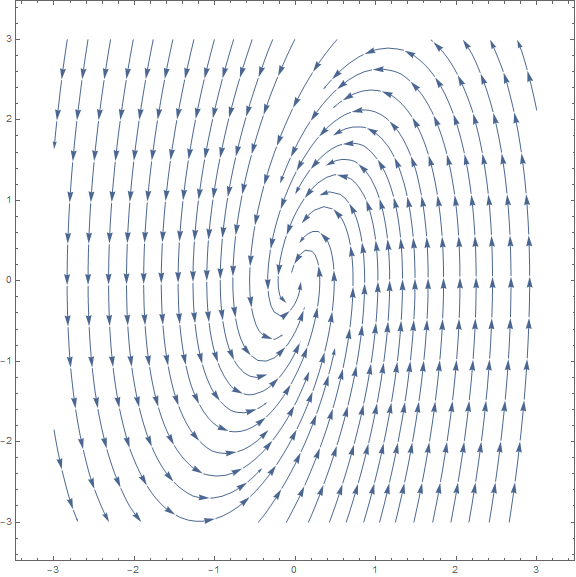
\includegraphics[scale=0.48]{graph9.2.png}} 
\end{center}

\textbf{Задача 2.} Решить систему дифференциальных уравнений методом вариации постоянной:
\begin{equation}
\left\{
\begin{array}{lr}
\dot{x}=x+2y+e^t\\
\dot{y}=2x+y+1
\end{array}
\right.
\end{equation}

\textbf{Решение:} 

1) Найдем решение однородной системы:
\[\left(
\begin{array}{c}
\dot{x}\\
\dot{y}
\end{array}\right)=
\left(
\begin{array}{cc}
1 & 2 \\
2 & 1
\end{array}\right)
\left(
\begin{array}{c}
x\\
y
\end{array}\right)\]
Собственные значения и собственные векторы:
\[(1-\lambda)^2-4=0\]
\[\lambda_1=-1, \;\;\; v_1=\left(
\begin{array}{c}
1\\
-1
\end{array}\right)\]
\[\lambda_2=3, \;\;\; v_2=\left(
\begin{array}{c}
1\\
1
\end{array}\right)\]

2) Диагональная матрица имеет вид:
\[D=\left(
\begin{array}{cc}
-1 & 0\\
0 & 3
\end{array}\right)\]
Матрица соственных векторов
\[C=\left(
\begin{array}{cc}
1 & 1\\
-1 & 1
\end{array}\right)\]
и обратная к ней матрица
\[C^{-1}=1/2\left(
\begin{array}{cc}
1 & -1\\
1 & 1
\end{array}\right)\]
Тогда общее решение задачи Коши имеет вид:
\[\left(
\begin{array}{c}
x(t)\\
y(t)
\end{array}\right)=C
\left(
\begin{array}{cc}
e^{-t} & 0\\
0 & e^{3t}
\end{array}\right)C^{-1}
\left(
\begin{array}{c}
x_0\\
y_0
\end{array}\right)\]
\[\left(
\begin{array}{c}
x(t)\\
y(t)
\end{array}\right)= \frac 1 2
\left(
\begin{array}{cc}
e^{-t}+e^{3t} & -e^{-t}+e^{3t}\\
-e^{-t}+e^{3t} & e^{-t}+e^{3t}
\end{array}\right)
\left(
\begin{array}{c}
x(t)\\
y(t)
\end{array}\right)\]
Для метода вариации постоянной систему удобнее записать в виде:
\[\left(
\begin{array}{c}
x(t)\\
y(t)
\end{array}\right)=
\left(
\begin{array}{cc}
e^{-t} & e^{3t}\\
-e^{-t} & e^{3t}
\end{array}\right)\left(
\begin{array}{c}
C_1\\
C_2
\end{array}\right)\]
\[x(t)=C_1(t)e^{-t}+C_2(t)e^{3t}\]
\[y(t)=-C_1(t)e^{-t}+C_2(t)e^{3t}\]
Продифференцируем x(t) и y(t):
\[\dot{x(t)}=\dot{C_1}e^{-t}-e^{-t}C_1+\dot{C_2}e^{3t}+3C_2e^{3t}\]
\[\dot{y(t)}=-\dot{C_1}e^{-t}+C-1e^{-t}+\dot{C_2}e^{3t}+3C_2e^{3t}\]
Подставим это в условие задачи (11.2):
\[\left(
\begin{array}{cc}
e^{-t} & e^{3t}\\
-e^{-t} & e^{3t}
\end{array}\right)\left(
\begin{array}{c}
\dot{C_1}\\
\dot{C_2}
\end{array}\right)=\left(
\begin{array}{c}
e^{t}\\ 
1
\end{array}\right)
\]
Отсюда найдем $C_1$ и $C_2$:
\[\dot{C_1}=\frac 1 2 (e^{2t}-e^t)\]
\[C_1=\frac1 4e^{2t}-\frac 1 2e^t\]
\[\dot{C_2}=\frac 1 2e^{-3t}+\frac 1 2e^{-2t}\]
\[C_2=-\frac 1 6e^{-3t}-\frac 1 4e^{-2t}\]
Тогда ответ:
\[x(t)=C_1e^{-t}+C_2e^{3t}-\frac 2 3\]
\[y(t)=-\frac 1 2 e^t+ \frac 1 3 - C_1e^{-t}+C_2e^{3t}\]
\textit{Примечание.} Эта задача также решалась и методом неопределенных коэффициентов как сумму частного и общего решения (причем решение таким способом оказывается чуть быстрее). Для этого необходимо искать частное  решение в виде
\[x(t)=ae^t+b\]
\[y(t)=ce^t+d\]
Несложно проверить, что ответ совпадает с полученным выше.

\markright{Дифференциальные уравнения. Семинар № 10}
\chapter[{Семинар №10}]{Семинар №10}
\thispagestyle{empty}

\textbf{Задача 1.} Решить систему дифференциальных уравнений: 
\begin{equation}
\left\{
\begin{array}{lr}
\dot{x}=y\\
\dot{y}=-x+x^3
\end{array}
\right.
\end{equation}
\textbf{Решение:}\\

1. Найдем стационарные точки:\[
\left\{
\begin{array}{lr}
0=y\\
0=-x+x^3
\end{array}
\right.\]
Стационарные точки: $(0, 0), (1, 0), (-1, 0)$

2. Линеаризация в окрестности каждой точки
\[\left\{
\begin{array}{lr}
\dot{x}=f(x,y)\\
\dot{y}=g(x,y)
\end{array}
\right.\]
\[\left(
\begin{array}{c}
\dot{x}\\\\
\dot{y}
\end{array}\right)=
\left(
\begin{array}{cc}
\frac{\partial f}{\partial x} & \frac{\partial f}{\partial y} \\\\
\frac{\partial g}{\partial x} & \frac{\partial g}{\partial y}
\end{array}\right) _{(x_0, y_0)}
\left(
\begin{array}{c}
x\\\\
y
\end{array}\right)\]

I) (0; 0)
\[\left(
\begin{array}{c}
\dot{x}\\
\dot{y}
\end{array}\right)=
\left(
\begin{array}{cc}
0 & 1 \\
-1 & 0
\end{array}\right) 
\left(
\begin{array}{c}
x\\
y
\end{array}\right)\]
Тип стационарной точки в ее окрестности:
\[\lambda^2+1=0\]
$\lambda=\pm i$ -- центр для линейной системы. Для нелинейной системы -- неизвестно.

II) $(1, 0), (-1, 0)$
\[\left(
\begin{array}{c}
\dot{x}\\
\dot{y}
\end{array}\right)=
\left(
\begin{array}{cc}
0 & 1 \\
2 & 0
\end{array}\right) 
\left(
\begin{array}{c}
x\\
y
\end{array}\right)\]
Тип стационарной точке в ее окрестности:
\[\lambda^2-2=0\]
$\lambda=\pm \sqrt{2}$ -- седло. Стационарные точки не устойчивы

3. Первый интеграл системы:
\[ \frac {dy} {dx} = \frac {-x+x^3} {y}\]
\[ y^2+x^2- \frac {x^4} 2 = C\]
Найдем значения констант в стационарных точках:
\[ (0,0): \;\;\; C=0\]
\[ (1, 0): \;\;\; C= \frac 1 2 \]
\[ (-1, 0): \;\;\; C= \frac 1 2 \]
По теореме о неявной функции функция (являющаяся сепаратрисой для периодичных решений) ниже является гладкой кривой всюду (кроме стационарных точек). 
\[ y^2+x^2- \frac {x^4} 2 = \frac 1 2\]

4. Изобразим фазовый портрет решений:
\begin{center}
{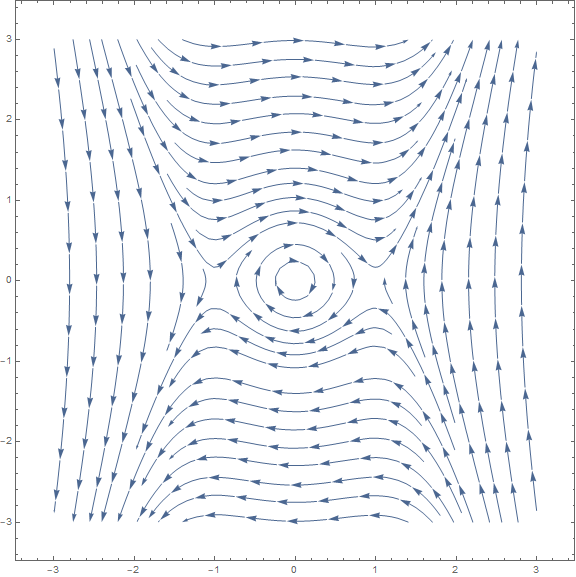
\includegraphics[scale=0.4]{graph12.1.png}} 
\end{center}
Заметим, что точка (0,0) имеет вид центра и устойчива по Ляпунову. Решения для $0<C<1/2$ периодичны (т.к. на них нет стационарных точек).
\section {Модель <<Хищник--жертва>> (Модель Лотки-Вольтерры)}
\textbf{Задача 2.} Решить систему дифференциальных уравнений, описывающих модель взаимодействия двух видов типа «хищник — жертва», где $x -$ популяция хищников, $y -$ популяция жертв.
\begin{equation}
\left\{
\begin{array}{lr}
\dot{x}=(-a+by)x\\
\dot{y}=(c-kx)y
\end{array}
\right.
\end{equation}
С параметрами $a,b,c,k>0$ и условиями $x(t) \geq 0, \;  y(t) \geq 0$\\
\textbf{Решение:}

Подробнее об истории модели и ее применимости можно почитать, например, \href{https://nplus1.ru/material/2019/12/04/lotka-volterra-model}{ в статье на сайте N+1} (кроме того, там же есть интерактивные графики с зависимостью системы от ее параметров, советую заглянуть туда). Здесь же сразу перейдем  к решению системы.

1. Стационарные точки:\\
\[\left\{
\begin{array}{lr}
0=(-a+by)x\\
0=(c-kx)y
\end{array}
\right.\; \Leftrightarrow \; (0, 0), \;\; \left(\frac c k, \frac a b\right)\]

2.Рассмотрим особые случаи начальных данных:\\
 $y_0=0$
\[\left\{
\begin{array}{lr}
\dot{x}=-ax\\
\dot{y}=0
\end{array}
\right.\]
\[y=y_0=0, \;\;\;\; x=x_0e^{-a(t-t_0)}\]
\[x_0=0 \Rightarrow x=x_0=0,\;\;\;\; y=_0e^{c(t-t_0)}\]
Т.е. оси -- тоже траектории движения.

3. Линеаризуя систему в окрестности точки (0,0), отметим, что она является центром, т. е. по теореме о линеаризации никакого вывода сделать нельзя.
 
4. Первый интеграл:
\[ \frac {dy} {dx} = \frac {y(c-kx)} {(by-a)x)}\]
Интегрируя, найдем его значение:
\[x^ce^{-kx-by}y^a=C\]
Градиент первого интеграла зануляется в стационарной точке $\left(\frac c k, \frac a b\right)$. По теореме о неявной функции это гладкие кривые (кроме стационарной точки). 

5. Изобразим фазовый портрет решений:
\begin{center}
{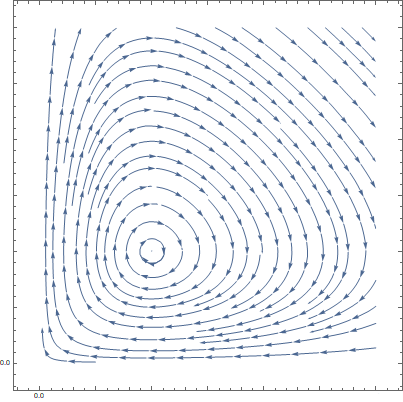
\includegraphics[scale=0.8]{graph12.2.png}} 
\end{center}
Стационарная точка $\left(\frac c k, \frac a b\right)$ устойчива по Ляпунову.

6. Все решения периодичны. 
\[y(t) = \frac 1 b \left( \frac {\dot{x}} {x} +a\right)\]
\[x(t) = -\frac 1 k \left( \frac {\dot{y}} {y} -c \right)\]
Проинтегрируем по периоду:
\[\int_{0}^{T} y(s) ds= \frac 1 b \int_{0}^{T}\left( \frac {\dot{x(s)}} {x(s)} ds+a\right)= \frac 1 b ln\; x(s) \big|_0^T+\frac a b T= \frac a b T\]
\[\frac 1 T \int_{0}^{T} y(s) ds= \frac a b \]
\[\frac 1 T \int_{0}^{T} x(s) ds= \frac c k \]
Интересный вывод: среднее значение популяции по периоду равняется стационарному значению.

7. Эффект рыбаков (harvesting).\\
Введем в нашу модель дополнительное условие: отлов обеих популяций с одинаковой интенсивностью, т.е.
\begin{equation}
\left\{
\begin{array}{lr}
\dot{x}=(-a+by)x-hx\\
\dot{y}=(c-kx)y-hy
\end{array}
\right.
\end{equation}
\[
\left\{
\begin{array}{lr}
\dot{x}=(-(a+h)+by)x\\
\dot{y}=((c-h)-kx)y
\end{array}
\right.\]
\[ a \rightarrow a+h \;\;\;\; c \rightarrow c-h\]
Таким образом, эффект рыбаков идет на руку жертве: среднее количество жертв увеличивается, а хищников -- уменьшится.

\textbf{Задача 2.} Решить систему дифференциальных уравнений:
\begin{equation}
\left\{
\begin{array}{lr}
\dot{x}=2y(y-2x)\\
\dot{y}=(1-x)(y-2x)
\end{array}
\right.
\end{equation}
\textbf{Решение:}

1. Стационарные точки:
\[ (1, 0), \{(x,y):= y=2x\}\]

2. \textit{Домашнее задание: определить характер точки (1, 0)}

3. Первый интеграл:
\[\frac {dy} {dx} = \frac {1-x} {2y}\]
\[y^2+ \frac {(x-1)^2} {2} = C\]
Кривые -- эллипсы.
\begin{center}
{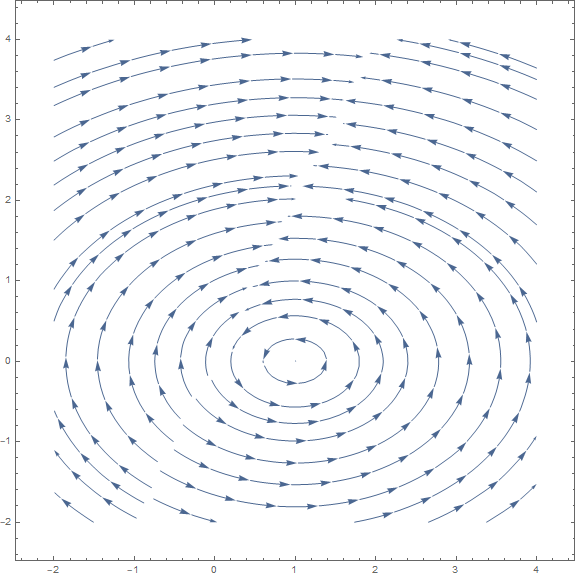
\includegraphics[scale=0.48]{graph12.3.png}} 
\end{center}
Линии уровня -- замнутые гладкие кривые, но периодических решений нет, т.к. нельзя зайти за стационарную точку. Все эти стационарные точки на прямой не являются устойчивыми. 

\chapter[{Семинар №11}]{Семинар №11}
\markright{Дифференциальные уравнения. Семинар №11}
\thispagestyle{empty}
\section {Модель SIR (Susceptible, Infected, Recovered)}
\textbf{Задача 1.} Решить систему дифференциальных уравнений (Задача Коши), описывающих модель распространения инфекции SIR (Susceptible, Infected, Recovered):
\begin{equation}
\left\{
\begin{array}{lr}
\dot{x}=axy-bx\\
\dot{y}=-axy
\end{array}
\right.
\end{equation}
где x(t) - infected и y(t) - susceptible, с начальными данными
\begin{equation}
\left\{
\begin{array}{lr}
x(0)=x_0\\
y(0)=y_0
\end{array}
\right.
\end{equation}
с параметрами $a,b>0$ и условием $x(t),y(t) \geq 0$.\\


\textbf{Решение:}

Опять же, во введении к решению задачи добавляю ссылку \href{https://nplus1.ru/material/2019/12/26/epidemic-math}{на статью с сайта N+1}, где хорошо расписаны условия применимости такой модели, есть симулятор распространения инфекции, наглядные графики и история возникновения такой модели. Кроме всего прочего, в статье разобраны модели SIS и MSEIR, более сложные, обширные и интересные системы уравнений, советую заглянуть :)

Теперь перейдем к решению нашего дифференциального уравнения.\\
1. Общее число популяции до начала эпидемии
\[x_0+y_0:=N\]
Проинтегрировав уравнения на y(t) и x(t), заметим, что из условия $x_0,y_0>0\;\Rightarrow x(t),y(t)>0\; \forall t$.Отсюда вывод: количество зараженных никогда не будет равно 0, если в начальный момент есть хоть какое-то число зараженных, т.е. эпидемия длится всегда (для достаточно большой популяции). Теперь посмотрим на следующую функцию:
\[N(t):=x(t)+y(t)\]
\[N(0)=N=x_0+y_0 \]
\[\dot{N}=\dot{x}+\dot{y}=-bx\leq 0 \;\; \Rightarrow \;\; N(.)   \downarrow \]

2. Существование решений по времени:
\begin{center}
{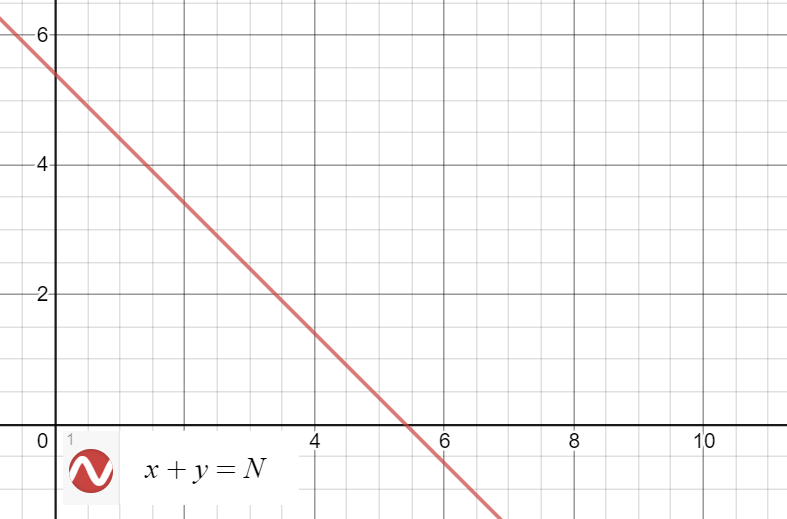
\includegraphics[scale=0.48]{graph13.1.png}} 
\end{center}
Обозначим треугольник за (T). Т.к. N(t) строго убывает, то 
\[x(t), y(t) \in (T), t>0 \Rightarrow\]
Все решения ограничены. Тогда интервал существования решений не ограничен. Решения существуют на $(-t^*, +\infty)$ (По теореме о максимальном интервале сущ. решения). Заметим, что решения не могут пересечь границу $x=y=0,$ т. к. решения не должны пересекаться.

3. Первый интеграл системы:
\[\frac {dy} {dx} = \frac {-axy} {axy-bx}\]
\[x=-y+\frac a b ln \; y +C\]
$\frac {dx} {dy}  = \frac {axy-bx} {-axy}> 0,$ если $y< \frac b a $\\


4. Стационарные решения:
 \[ \left\{
\begin{array}{lr}
0=axy-bx\\
0=-axy
\end{array}
\right. \Rightarrow\]
\[(0;0), (0, \xi) \;\; \forall \xi\]
Т.е. стационарные решения: вся прямая $x=0$. В условиях модели: инфицированных нет. Рассмотрим 2 случая:\\
I) $y_0> \frac b a$\\
II) $y_0 \leq \frac b a \; \Rightarrow \; x(t) \downarrow$.  Первый интеграл строго убывает. 
$\frac b a$-- порог развития эпидемии. Если количество инфицированных не превышает этого порога, то эпидемия не разовьется, и количество инфицированных будет убывать.

Найдем $x_{max}$:
\[x'_y=0=-1+ \frac {b} {ay}=0 \]
\[y= \frac b a \]
\[x_{max}=- \frac b a +\frac b aln\;\frac b a +C\]
$\dot{y(t)}<0$ -- y строго убывает. Тогда существует предел при $t\rightarrow+\infty$. 
\[\dot{y}=-axy\]
\[y(t)=y_0e^{a\int^t_0x(s)ds}\] 
\[\dot{N}=\dot{x}+\dot{y}=-bx\]
\[-b\int^t_0x(s)ds=N(t)-N(0)=x(t)+y(t)-N\]
\[b\int^t_0x(s)ds \leq N\]
\[-a\int^t_0x(s)ds \geq -\frac {Na} {b}\]
Следовательно, $\lim_{t\to+\infty} y(t)=y_{\infty}>0$. Т. е. неиммунизированный остаток популяции всего больше 0.
Для x верно следующее:
\[\int^t_0x(s)ds\leq \frac {x_0+y_0} {b}\]
Т.к. этот интеграл ограничен для любого t,  $\lim_{t\to+\infty} x(t)=0.$
График решений дифференциального уравнения (здесь $ a=b=1$):
\begin{center}
{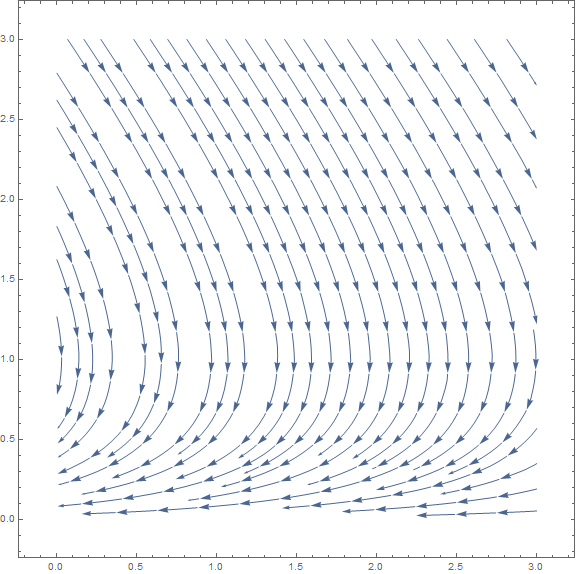
\includegraphics[scale=0.48]{graph13.2.png}} 
\end{center}

\section {Уравнение математического маятника}
\textbf{Задача 2.} Решить дифференциальное уравнение (математический маятник без трения):
\begin{equation}
\ddot{z}+\frac g l sin\;z=0
\end{equation}

\textbf{Решение:}

1.Перейдем к системе. Сделаем замену:
\[ \left\{
\begin{array}{lr}
x=z\\
y=\dot{z}
\end{array}
\right.\]
Тогда получим систему 
\[ \left\{
\begin{array}{lr}
\dot{x}=y\\
\dot{y}=- \frac g l sin\;x
\end{array}
\right.\]

2. Стационарные точки:\\
$(\pi n,0), \; n\in \textbf{Z}. $ Так как система периодична, достаточно рассмотреть 2 стационарные точки: $(0,0), (\pi,0)$

3. Линеаризация в окрестности стационарных точек и исследование типа:

I) $(0,0)$
\[ \left\{
\begin{array}{lr}
\dot{x}=y\\
\dot{y}=- \frac g l
\end{array}
\right.\;\;\Rightarrow\]
Характеристический многочлен:
\[\lambda^2+\frac g l =0\]
\[\lambda=\pm i \sqrt{\frac g l }\]
Картина -- центр. Есть устойчивость по Ляпунову (но нет асимптотической устойчивости). Для исходной системы -- теорема ничего не говорит об устойчивости. \\
II) $(\pi,0)$
\[ \left\{
\begin{array}{lr}
\dot{x}=y\\
\dot{y}= \frac g l
\end{array}
\right.\;\;\Rightarrow\]
\[\lambda^2-\frac g l =0\]
\[\lambda=\pm  \sqrt{\frac g l }\]
Картина -- седло, устойчивости нет. Для исходной системы -- точка неустойчива. 

4. Первый интеграл системы:
\[ \frac {dy} {dx}= \frac{-gsin\;x}{ly}\]
\begin{equation}
\frac 1 2 y^2=C+\frac g l cos\; x
\end{equation}

5. Изобразим график $-U(x)=cos\;x$ и различные значения C (положим $\frac g l = 1$):
\begin{center} 
{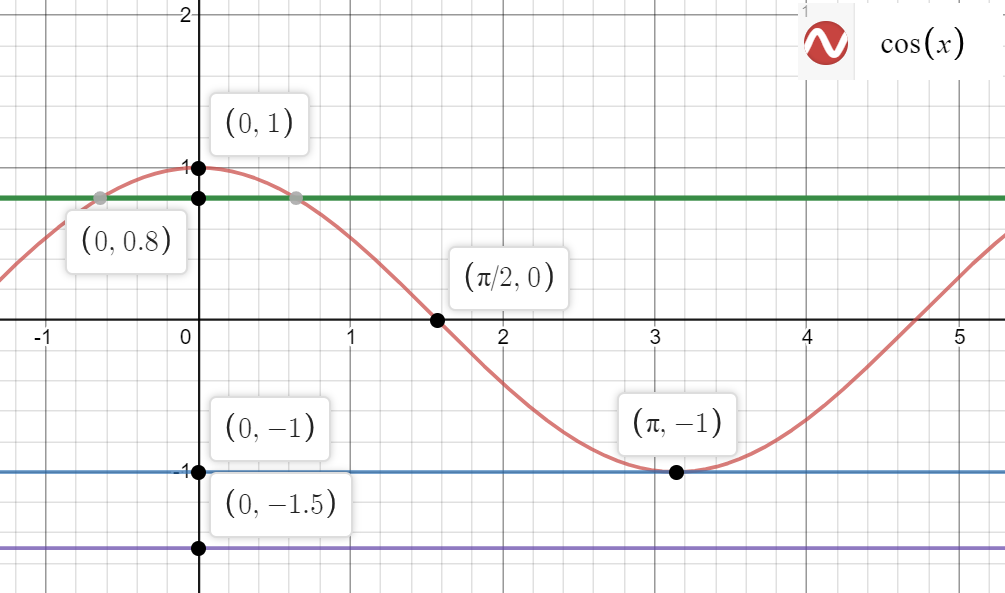
\includegraphics[scale=0.48]{graph13.3.png}} 
\end{center}
Рассмотрим различные C. \\
a) Пусть $C=-1.$ Тогда (13.4) разрешимо при $cos\;x=1$. Линии уровня -- точки. \\
b) Пусть $C=-1+\varepsilon,\; \varepsilon >0$. Линии уровня -- центры (периодические замкнутые траектории, устойчивость сохраняется).\\
c) Пусть $С=1.$ Тогда выражая y из (13.4) и раскладывая косинус, то получаем $y^2=x^2$. Траектории замыкаются.\\
d) Пусть $C=1+\varepsilon,\; \varepsilon >0 (\varepsilon$ здесь не обязательно мало). Получаем непериодические траектории.\\
Направление траекторий определяются по знаку производной в какой-либо точке. 

6. Тогда можем изобразить фазовый портрет системы:\\
P.s.Наглядная демонстрация движения маятника доступна \href{http://math-info.hse.ru/f/2015-16/nes-ode/pendulum.html}{на сайте Ильи Щурова}.
\begin{center} 
{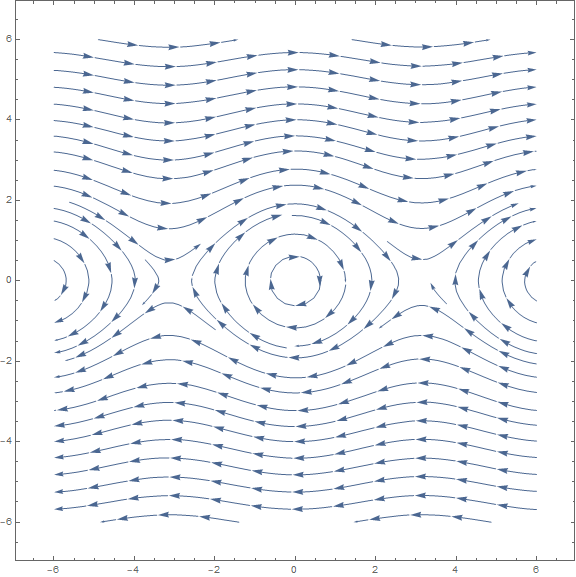
\includegraphics[scale=0.66]{graph13.4.png}} 
\end{center}

7.Периодические решения:

\[x(t)=x(t+T)\]
\[y(t)=y(t+T)\]
\[\frac 1 2 y_0^2<1+\frac g l cos\; x_0\]
Сепаратриса при $C=1 $ разделяет периодические и непериодические решения. 

8. \textit{Небольшое дополнение:} маятник с трением ($k\ll 1$)\\
После соответствующих замен уравнение маятника
\[\ddot{z}++k\dot{z}+\frac g l sin\;z=0\]
сводится к системе:
\[ \left\{
\begin{array}{lr}
\dot{x}=y\\
\dot{y}=- \frac g l sin\;x-ky
\end{array}
\right.\]
Рассмотрим поведение особых точек в этом случае:
a)\[-\lambda(-\lambda-k)+\frac g l =0\]
\[D=k^2-4\frac g l \]
Комплексные корни, значит, особая точка -- фокус.
b)\[\lambda^2+k\lambda-\frac g l =0\]
Особая точка -- седло.\\
Фазовый портрет для маятника с трением имеет вид:
\begin{center} 
{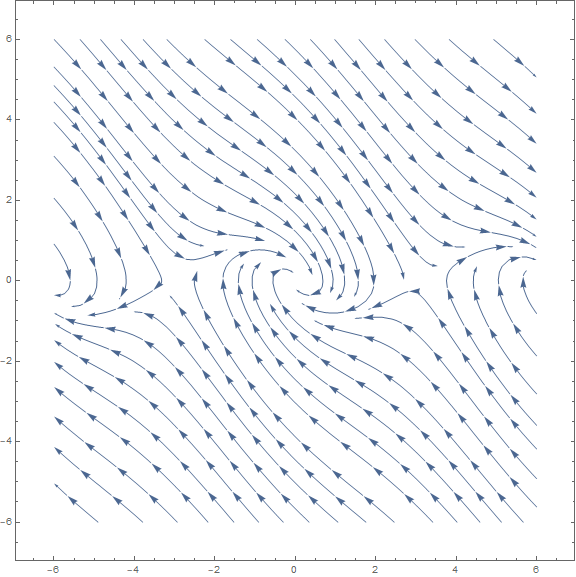
\includegraphics[scale=0.6]{graph13.5.png}} 
\end{center}

\textbf{Задача 3.} Решить систему дифференциальных уравнений:
\begin{equation}
\left\{
\begin{array}{lr}
\dot{x}=-y+x(1-\sqrt{x^2+y^2})\\
\dot{y}=x+y(1-\sqrt{x^2+y^2})
\end{array}
\right.
\end{equation}

\textbf{Решение:}

1. Перейдем к полярной системе координат:
\[x=r\;cos\;\varphi,\;\;\;y=r\;sin\;\varphi\]
\[\dot{x}=\dot{r}cos\;\varphi-rsin\;\varphi\;\dot{\varphi}\]
\[\dot{y}=\dot{r}sin\;\varphi+rcos\;\varphi\;\dot{\varphi}\]
Тогда исходная система (13.5) эквивалентна следующей:
\[\left\{
\begin{array}{lr}
\dot{r}=r(1-r)\\
\dot{\varphi}=1
\end{array}
\right.\]

2. Стационарные точки (у исходной системы):
\[x=0\;\;\;\; y=0\]
При $r\rightarrow 0,\; \dot{r}=r,\; \varphi=1$

3. Линеаризация в точке $(0,0)$:
\[\dot{x}=-y+x\]
\[\dot{y}=x+y\]
Получаем неустойчивый фокус.
\[ r= 1, \dot{\varphi}=1\]
Получили предельный цикл. Траектории внутри цикла стремятся к этому циклу. При больших r:
\[\dot{r}=-r^2\]
Наоборот приближаемся к началу координат, т.е. стремимся к предельному циклу.

4. Первый интеграл:
\[ \frac {dr}{d\varphi}=r(1-r)\]
\[\frac {r} {1-r}=Ce^{\varphi}\]
$r=1$ -- устойчивое периодическое решение.\\
Изобразим фазовый портрет:
\begin{center} 
{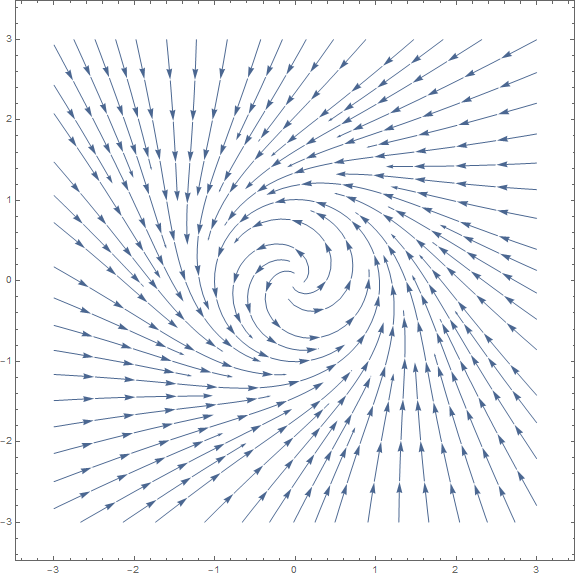
\includegraphics[scale=0.6]{graph13.6.png}} 
\end{center}

\chapter[{Семинар №12}]{Семинар №12}
\markright{Дифференциальные уравнения. Семинар №12}
\thispagestyle{empty}
\section {Простейшая система управления в дифференциальных уравнениях}
\textbf{Задача 1.} Есть динамика взаимоотношений:
\begin{equation}
\left\{
\begin{array}{lr}
\dot{x}=y\\
\dot{y}=-x
\end{array}
\right.
\end{equation}
Система -- гармоничекий осциллятор, его решение давно нам известно. Также известно, что $x^2+y^2=x_0^2+y_0^2$, фазовые траектории -- окружности, устойчивости нет. Тогда поставим перед собой задачу: подобрать функцию управления $u(x)$ такую, что система 
\begin{equation}
\left\{
\begin{array}{lr}
\dot{x}=y\\
\dot{y}=-x+u(x)
\end{array}
\right.
\end{equation}
стабилизировалась бы,  то есть $x(t), y(t) \rightarrow 0$ при $t\rightarrow+\infty$.\\

\textbf{Решение:}\\
\textit{Нетривиальный ответ}: ничего не выйдет. Докажем это. \\
Введем функцию 
\[ V(x,y):=y^2-2\int^x_0(-r+u(r))dr\]
Посчитаем производную Ли вдоль направления траекторий системы (14.2) этой функции:
\[\frac {d} {dt} V= 2y\dot y -2(-x+y(x))\dot x =2y(-x+u(x))-2(-x+u(x))y=0\]
Выходит, что $V(x(t),(y(t))=const$. Если бы выполнялось $x(t), y(t) \rightarrow 0$, то $V(x(t),(y(t))\rightarrow 0$ при $t\rightarrow+\infty$. Противоречие. Стабилизировать систему нельзя.

Теперь введем следующую модель управления. Изменение управления будет происходить только в дискретные моменты времени T. $b\ll1$ . Изначально u=0. В зависимости от знака $x(t)$ происходит изменение модели:
\begin{center} 
{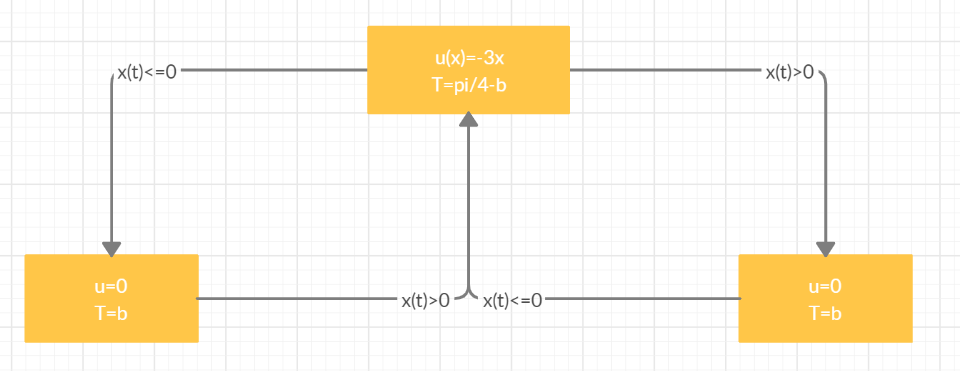
\includegraphics[scale=0.5]{graph14.1.png}} 
\end{center}
Такое управление будет систему стабилизировать. Рассмотрим пример, изображенный на графике. Из начальной траектории (красной), переходим к системе с $u(x)=-3x$, описывающую движение по эллипсу (синяя траектория). Т.к. после T мы все равно остаемся в первом квадранте, то движение снова изменяется и переходит на новую траекторию с  $u(x)=0$ (зеленая окружность). Система находится в состоянии с $u(x)=-3x$ примерно $T= \frac {\pi} 4$.
\begin{center} 
{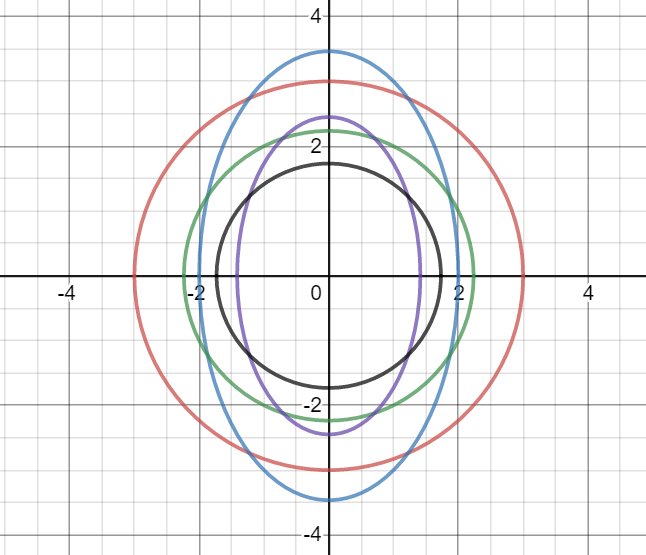
\includegraphics[scale=0.5]{graph14.2.png}} 
\end{center}
Можно посчитать, что за раз радиус меняется в $\sqrt3/2$ раз. Так мы получаем, что  $x(t), y(t) \rightarrow 0$ при $t\rightarrow+\infty$.

Однако выше мы отметили, что стабилизировать систему нельзя. В чем противоречие?\\
Дело в том, что описанная система уже не будет являться обыкновенным дифференциальным уравнением. Если мы возьмем два начальных данных на одной окружности, тогда обе траектории могут упасть на одну и ту же окружность в результате действия управления. Тогда возможен случай, когда моменты контроля совпадут -- траектории сольются в конечный момент времени, и единственности решений не будет. Тогда никаких противоречий нет.

Описанная же система называется гибридным управлением. 


\markright{Консультация перед контрольной работой №3}
\chapter[{Консультация перед контрольной работой №3}]{Консультация перед контрольной работой №3}
\thispagestyle{empty}
\textbf{Задача 1.} Решить систему дифференциальных уравнений:
\begin{equation}
\left\{
\begin{array}{lr}
\dot{u}=v-u^2v-v^3\\
\dot{y}=u^2+v^2-1
\end{array}
\right.
\end{equation}

\textbf{Решение:}

1. Стационарные точки
\[\left\{
\begin{array}{lr}
\dot{u}=v-u^2v-v^3\\
\dot{y}=u^2+v^2-1
\end{array}
\right.\]
Множество стационарных точек: $\{(u_0,v_0):\; u_0^2+v_0^2=1\}$

2. Линеаризация в окрестности точки:
\[A=\left(
\begin{array}{cc}
2u_0v_0 & 1-u_0^2-3v_0^2\\
2u_0 & 2v_0
\end{array}\right)\]

Корни соответствующего характеристического многочлена:
\[\lambda_1=0 \;\;\; \lambda_2=2v_0(1-u_0)\]
Если $\lambda_2=2v_0(1-u_0)>0,$ то положение равновесия неустойчиво, т.е. точки, лежащие на части окружности  $u_0^2+v_0^2=1, v>0$ неустойчивы.

3. Первый интеграл:
\[ \frac {du}{dv}=-v,\; \; u^2+v^2\ne1\]
\[u=- \frac {v^2} 2 +c\]

4. Определим направления движения (при прохождении через стационарную точку меняется знак производной). Особый интерес представляет парабола с C=1. Рассматривая систему уравнений "окружность+гипербола", определяем, что есть только одна точка касания (1,0).
\begin{center}
{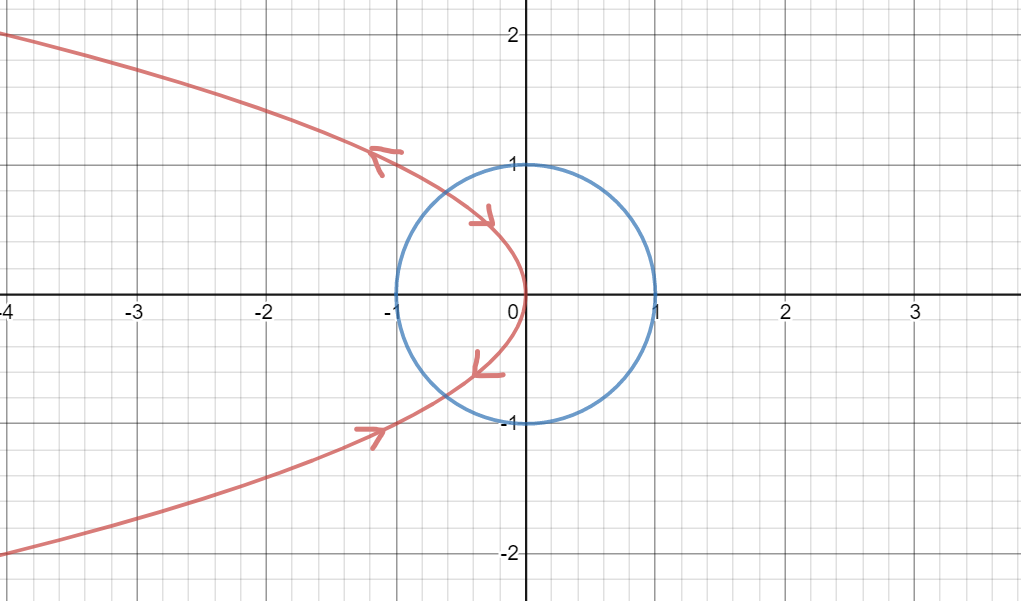
\includegraphics[scale=0.35]{graph15.2.png}} 
\end{center}

5. Устойчивость.\\
Как уже было отмечено выше, точки $u_0^2+v_0^2=1, v>0$ неустойчивы. \\
Рассмотрим точки на нижней дуге. Действуем по определению: для $x_0$ находим пересечение $\varepsilon$  с единичной окружностью, находим крайние траектории, входящие в эту окрестность и выбираем $\delta<min(z-x_0)$, где z -- точка на этой траектории. Асимптотической устойчивости нет. \\
Стационарные точки на прямой v=0, очевидно, не являются устойчивыми.
  
6. Периодичность решений.\\
Периодических решений здесь нет (если не считать стационарные точки частными случаями периодических с любым периодом), нет замкнутых траекторий. 

7. Наконец, изобразим фазовый портрет:
\begin{center}
{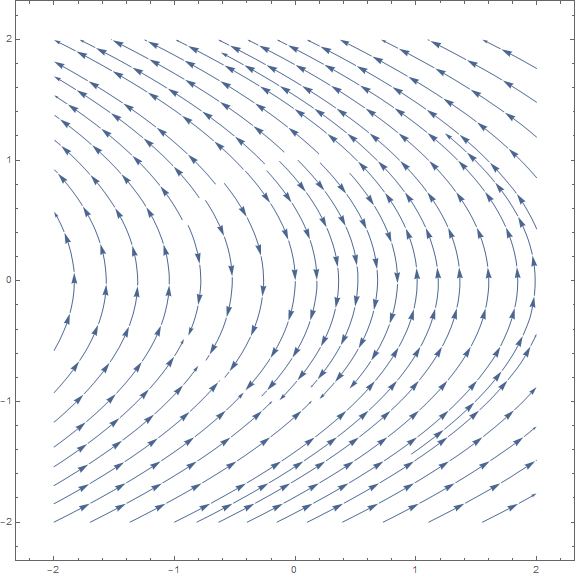
\includegraphics[scale=0.4]{graph15.1.png}} 
\end{center}
\end{document}
